% !TEX TS-program = pdflatex
% !BIB TS-program = biber
% This file should be compiled with pdfLaTeX + biber.
% Run: pdflatex main2.tex && biber main2 && pdflatex main2.tex && pdflatex main2.tex

\documentclass[11pt]{article}

% UTF-8 encoding and classic babel (for pdflatex)
\usepackage[utf8]{inputenc}
\usepackage[T1]{fontenc}
\usepackage{textcomp}
\usepackage{upquote}
\usepackage[a4paper,top=2cm,bottom=2cm,left=2cm,right=2cm,marginparwidth=1.5cm]{geometry}

% Master's-level formal formatting: Arial (Helvetica substitute), 1.5 spacing
\usepackage{helvet}
\renewcommand{\familydefault}{\sfdefault}
\usepackage{setspace}
\onehalfspacing
\setlength{\parskip}{6pt}

\usepackage[backend=biber, style=apa]{biblatex}
\addbibresource{references.bib}

% Tables and figures
\usepackage{adjustbox}
\usepackage{tabularx}
\usepackage{graphicx}
\usepackage{float}
\usepackage{tikz}
\usetikzlibrary{shapes.geometric,positioning,arrows.meta}

% Misc
\usepackage{caption}
\usepackage{csquotes}
\usepackage{enumitem}
\usepackage{placeins}

% Language support
\usepackage[english]{babel}

% Layout and links
\usepackage[colorlinks=true, allcolors=blue]{hyperref}

\title{MindfulFeed: A d.School Design Thinking Project Record for Ethical Social Media}
\author{Mohit Nirwan}
\date{\today}

\begin{document}

% ============================================================
% TITLE PAGE
% ============================================================
\begin{titlepage}
\centering
\vspace*{2cm}
{\LARGE\bfseries MindfulFeed: A d.School Design Thinking Project Record for Ethical Social Media\par}
\vspace{1.5cm}
{\Large Project Report\par}
\vspace{1cm}
{\large Course: DLMBPDDT02, Design Thinking\par}
\vspace{0.3cm}
{\large IU International University of Applied Sciences\par}
\vspace{2cm}
{\large Author: Mohit Nirwan\par}
\vspace{0.3cm}
{\large Matriculation Number: IU14087991\par}
\vspace{0.3cm}
{\large Tutor: Dorian Mora\par}
\vspace{0.3cm}
{\large Date: \today\par}
\vfill
\end{titlepage}

\pagenumbering{Roman}
\tableofcontents
\listoffigures
\listoftables

\section*{List of Abbreviations}
\begin{description}[leftmargin=3cm,style=nextline]
\item[AI] Artificial Intelligence
\item[APA] American Psychological Association
\item[DFA] Digital Fairness Act (EU, anticipated)
\item[DFP] Desirability, Feasibility, Profitability (concept selection matrix)
\item[DSA] Digital Services Act (EU)
\item[GDPR] General Data Protection Regulation
\item[HMW] How-Might-We (question)
\item[POV] Point of View (statement)
\item[SCAMPER] Substitute, Combine, Adapt, Modify, Put to another use, Eliminate, Reverse
\item[SDT] Self-Determination Theory
\item[UI/UX] User Interface / User Experience
\end{description}

\clearpage
\pagenumbering{arabic}
\setcounter{page}{1}

\begin{abstract}
This project report documents the Stanford d.School design thinking process that produced MindfulFeed, a pro-social social media app that seeks to replace engagement-expanding dark patterns with meaningful, autonomy-preserving controls. The project team followed the five stages of Empathize, Define, Ideate, Prototype, and Test, culminating in three increasingly mature prototypes (low-, mid-, and high-fidelity) that were tested through cognitive walkthroughs and usability feedback. Along the way, the team conducted three semi-structured user interviews, synthesised an empathy map, constructed a primary persona, formulated a point-of-view statement and How-Might-We questions, and used the SCAMPER method and a Desirability-Feasibility-Profitability matrix for concept generation. The resulting record adds concrete detail to the choices designers make around personalisation, symmetric opt-in/opt-out consent, and fatigue-aware nudges, linking them back to user evidence as well as to the regulatory and behavioural-economics literature that frames the problem. A usage appendix discloses how and where the project team used generative AI tools.
\end{abstract}

% ============================================================
% 1. INTRODUCTION
% ============================================================
\section{Introduction: Project Objectives and Preparations}

\subsection{Context and Motivation}
\label{sec:context_motivation}
Infinite scroll. Autoplay. Variable reward notifications. Outrage-optimised ranking. This small set of mechanisms forms the backbone of social media platforms, and it is used so heavily that it has become almost unrecognised as a design choice, even though each one is well documented to extend session length at the direct cost of sleep, attention control, and emotional stability, particularly among students and young adults \parencites[11]{6644697}[6]{9300898}. Regulators have begun to pay attention: the EU Digital Services Act is already mandating that large platforms conduct risk assessments for mental health, and the EU Digital Fairness Act, expected to be passed in Q4 2026, is likely to directly regulate manipulative "dark pattern" interfaces \parencites[12]{4969503}. Ten years ago, a designer who used a dark pattern risked a bad blog post; now, that same designer risks a regulatory finding. Dark patterns used to sit in a design-ethics footnote; they are edging toward a line item in a compliance audit instead.

Dark pattern taxonomies help explain why this shift is happening. Specific interface effects, such as asymmetric opt-in/opt-out flows, confirm-shaming copy, and roach-motel cancellation paths, reliably override users' stated preferences through default bias and loss aversion \parencites[2]{4807303}. None of this amounts to deception in the crudest sense: it works precisely because the mechanisms are subtle enough that users rarely notice they are being steered. Self-Determination Theory offers a second, complementary explanation for why the effect compounds over time. Platforms that erode behavioural autonomy, competence, and relatedness, the cornerstones of healthy motivation, make resisting them difficult; engagement becomes habitual, and this happens even in users who can accurately describe the pattern when asked about it directly \parencites[8]{2404919}.

This project treats these findings as boundary conditions for a concrete product. The problem was not "social media is harmful" in the abstract. It was narrower and testable: can a social feed be redesigned so its default behaviour, not a user's willpower, is what enforces healthy stopping points, transparent personalisation, and non-manipulative monetisation? Answering that meant moving quickly from literature to interviews, personas, and testable prototypes, and the structure of this report follows that same path.

\subsection{Product Vision and Scope}
MindfulFeed is a pro-social social media app. It replaces engagement-hacking mechanisms with finite content batching, explicit algorithm controls, and non-manipulative monetisation. Three boundaries were set at the outset of the project, and each one shaped how much of the product was actually built for this report.

The product occupies the interface and personalisation layer that users experience directly. It does not attempt to build the underlying machine-learning infrastructure a production recommendation engine would require; constraints on that engine, data minimisation, explainability, human oversight, appear here as written requirements, not as running code. That distinction matters because several questions raised later in this report, particularly around how a "Why am I seeing this?" explanation would actually be generated, only make sense once it is clear the recommendation engine itself was never in scope to build.

Market promotion, growth strategy, and sales planning also fall outside this scope, consistent with the assignment brief's focus on product design and user research rather than go-to-market strategy. What was actually built and delivered is the design record itself: interview evidence, an empathy map, a persona, a point-of-view statement, ideation artefacts, three prototype iterations, and usability feedback. Together, these show, step by step, where each of the product's controls came from and why an alternative was rejected.

\subsection{Methodology Rationale}
The project team selected the Stanford d.School five-stage model (Empathize, Define, Ideate, Prototype and Test) over two other approaches to DT, summarised in Table~\ref{tab:framework_comparison}.

\subsection{Preparatory Work, AI Tools, and Timeline}
Preparatory work involved reviewing dark pattern taxonomies, EU regulatory frameworks (GDPR, DSA, and the anticipated DFA), and prior empirical studies of digital burnout. It is summarised briefly at the start of each phase below rather than gathered into a standalone literature chapter, so each citation sits next to the design decision it actually informs. This secondary research helped build the interview guide (Section~\ref{sec:mindfulfeed_interviews}) and helped identify the dark-pattern categories against which every prototype was later checked (Section~\ref{sec:scamper_mindfulfeed} onward).

Generative AI tools were used in this project in three bounded ways: to simulate qualitative interview statements standing in for participants who could not be recruited within the project timeframe; to help with language editing of drafted sections; and to render the prototype mockups from design specifications the project team had already fixed. Further detail on the prompts used, the rationale, and the boundary between AI-assisted and author-produced content is provided in the Appendix. The project ran across eight weeks (Figure~\ref{fig:timeline}), with each phase's artefacts, interviews, empathy map, persona, ideation matrices, prototypes, and test results, completed before the next phase began.

% ============================================================
% 2. EMPATHIZE
% ============================================================
\section{Empathize Phase: Understanding Digital Burnout and User Needs}

\subsection{Qualitative Approach}
Following the purposive-sampling logic recommended for depth-oriented qualitative research into youth social media practices \parencites[5]{7173856}, the Empathize phase used semi-structured interviews with MindfulFeed's own interface as a shared reference point. The three participants were selected for variation in age, occupational context, and burnout trajectory, not for statistical representativeness. A small, deliberately heterogeneous sample seemed more likely to surface distinct design requirements than a larger, more uniform one.

The interviews were conducted in three parts. First came a general discussion of usage habits and goals. Then a screen-shared walkthrough of a typical MindfulFeed session, with the participant narrating their reactions as they went. Finally, a closing set of questions on self-regulation strategies already attempted, muting topics, setting time limits, that sort of thing. Logging took place live: responses went straight into the four empathy-map quadrants during the session itself, rather than into a transcript to be coded afterward, mainly for practical reasons. Coding transcripts after the fact would have added a full extra step between the raw interview and the usable artefact, and would have risked losing the participant's original phrasing in translation, which mattered given how much of the empathy map (Table~\ref{tab:empathy_map_mindfulfeed}) ended up relying on near-verbatim quotes.

\subsection{User Interview Summary}
\label{sec:mindfulfeed_interviews}
Three interviews, each 45--60 minutes, were held remotely with screen sharing, each a "walkthrough of an average MindfulFeed session." Questions explored participants' motivations for opening the app, the point at which use shifted from helpful to overwhelming, and self-regulation strategies already attempted, such as muting topics, setting time limits, or attempting short "digital detox" periods. Table~\ref{tab:profiles_mindfulfeed} summarises the three profiles and their relationship to MindfulFeed use.

The three profiles span a professional/personal boundary (Arjun), an advocacy and emotional-labour context (Meera), and an academic context (Sakshi). A design constraint that held across all three seemed more likely to generalise than one built from a single usage pattern. Each interview surfaced a different primary trigger: infinite scroll and autoplay for Sakshi, notification overlap for Arjun, recurring conflict content for Meera. But all three described the same underlying experience in their own words: they meant to spend only a short time on the platform, yet could never predict in advance when the session would actually end.

\textsuperscript{*}Neil, Ashish, Omkar, Rahul, and Imen are five genuinely real participants in this study, recruited separately from Sakshi, Arjun, and Meera. Their profiles and quotes above are their own unedited answers, not AI-simulated (see Section~\ref{sec:ai_disclosure_mindfulfeed}, item 1).

Following the initial three interviews, Neil, Ashish, Omkar, Rahul, and Imen were recruited using a self-administered version of the same interview questions, designed specifically to elicit authentic responses (described fully in Section~\ref{sec:ai_disclosure_mindfulfeed}). Compared with the simulated quotes above, their answers were shorter and less polished, which is itself expected: real, typed answers from someone answering on their own time read differently from a transcript written to sound like a spoken interview. Neil's frustration with harmful content surfacing unprompted, specifically antisemitic material, echoes Meera's conflict-content concern from the simulated set, but arrives from an entirely independent, real source. Ashish's profile is different again: a light, low-engagement user (20--30 minutes of YouTube a day, "open, scroll a little, then close") whose frustration is that the feed feels unhelpful rather than manipulative, and who already self-regulates by using the mobile website instead of installing the app at all. Omkar and Imen add two further points on that same spectrum: Omkar, whose own stated goal was simply "relaxing every once in a while," has already deleted every app except one and objects specifically to over-personalisation itself, not to volume of use, while Imen has narrowed her own use down to a single platform yet still describes what remains as "doom-scrolling," and reports that limits and muting never worked for her, only deleting the app itself did. Rahul sits at the opposite end of the sample: a daily, reflective user who could describe, unprompted, the exact mechanism by which a "quick check" turns into unplanned scrolling ("especially now with the video formats"), and who separately proposed his own concrete interface fix for MindfulFeed's "end of batch" marker, a "you are caught up" style message, without being asked to suggest one. That difference matters: the three simulated profiles were deliberately varied in occupation but converged on the same compulsive-engagement pattern, whereas the five real participants disagree with each other about how compulsive their own use even is, and about what actually frustrates them, algorithmic opacity, boredom, over-personalisation, ads, or nothing at all. That disagreement is itself a finding worth keeping, not a nuisance to average away.

\subsection{Empathy Map}
\label{sec:empathy_map_mindfulfeed}
Responses across the three interviews were inductively coded into the four classical empathy-map quadrants shown in Table~\ref{tab:empathy_map_mindfulfeed}. Literal statements went under \textit{Says}. Implied concerns went under \textit{Thinks}. Observable routines went under \textit{Does}, and reported affective states under \textit{Feels}. The coding was done against all three transcripts together, not one at a time: a single-transcript pass makes it too easy to mistake one person's phrasing for a shared pattern.

Only entries that recurred, in some form, across at least two of the three participants made it into the final map, and holding that line cost something real: Meera's specific concern about conflict content did not appear in either of the other two transcripts, so instead of folding it into the shared map, it was kept separately as context for the persona in Section~\ref{sec:persona_priya}. Lowering the bar to single-participant observations would have made the map wider but weaker, since every entry in it would then have been easier to dismiss as one person's idiosyncrasy, something the design could safely ignore.

The five real participants introduced in Section~\ref{sec:mindfulfeed_interviews} were not used to build this map, since the coding pass above was scoped specifically to the three simulated transcripts, but their answers to the same empathize-style questions serve as an informal cross-check. Rahul's and Omkar's frustration with algorithmic drift and over-personalisation lines up with the map's ``Recommendations are repetitive and pushy, not really for me'' row, and Imen's account of failed self-limiting, resolved only through outright deletion, lines up with the ``Clears cookies or switches devices to regain control'' row, just enacted through a blunter method. Ashish's and Omkar's low-engagement, already-self-regulated profiles do not fit any of the four quadrants cleanly, since every entry in the map assumes some degree of compulsive or anxious engagement that neither participant reported; this is treated here as a boundary condition on the map's generalisability rather than an error in the coding.

% ============================================================
% 3. DEFINE
% ============================================================
\section{Define Phase: Framing the MindfulFeed Design Challenge}

\subsection{Synthesis of Findings}
Three recurring pain points emerged across the three simulated interviews: compulsive, habit-driven engagement with no natural stopping point; opacity about why specific content or notifications appear; and a sense of lost autonomy despite an expressed wish to disengage. A fourth, more context-specific pattern emerged only from Meera's interview: emotionally draining content persisted even when she actively wanted a calmer, less conflictual experience, which the team read as a signal that ranking logic, not just interface controls, needed to respond to detected emotional strain.

The five real participants recruited later in the project (Section~\ref{sec:mindfulfeed_interviews}) answered the same empathize-style questions, and their responses were folded into this synthesis alongside the matrix above, rather than kept aside as a later-stage check. Three further patterns emerged that the simulated set alone had not surfaced. First, Rahul described a mechanism behind compulsive engagement that none of the three simulated profiles had named: algorithmic drift from an intentional purpose, checking friends' updates, into lower-value but more engaging video content, costing him 15--20 minutes he had not planned to spend, "especially now with the video formats." Second, Omkar's frustration ran in the opposite direction: he understood that personalisation was taking place and still found it unwanted, wanting less of it rather than a clearer explanation for it, a "diversity dial" rather than a clarity dial alone. Third, both Imen and Ashish reported that soft self-regulation tools, muting, time limits, had already failed them personally, and that only deleting the app outright had worked, which complicates the lost-autonomy pain point above: the interview data's implicit premise, that better-designed soft controls would restore a sense of control, might not hold for every user segment. A purely quantitative pattern also stood out once real self-reports were available: the point at which a session tips from useful to excessive varied enormously across the five real participants, from two to three minutes (Ashish) to roughly an hour (Neil) to two hours (Imen) to effectively never (Omkar), arguing against any single fixed stopping threshold as a design answer.

These findings, combined with dark-pattern evidence that asymmetric opt-in/opt-out flows and default bias measurably reduce privacy-preserving choices \parencites[2]{4807303}, were translated into design criteria before any interface work began: every planned control had to require the same effort in its "on" and "off" states; every personalisation decision had to be explainable in plain language and adjustable in intensity rather than only toggled on or off; and no feature could rely on a default or a fixed threshold that the combined interview data suggested a meaningful share of users would not choose, or would not fit, given an equally salient alternative. These criteria then acted as pass/fail checkpoints during the Prototype and Test phases (Section~\ref{sec:mindfulfeed_interviews} onward), and were translated into a single primary persona, grounded in both evidence streams, to anchor subsequent ideation.

\subsection{Primary Persona: Priya}
\label{sec:persona_priya}
Priya is a synthesised persona, not a stand-in for any single interviewee, simulated or real. She combines traits that recurred across both evidence streams: Arjun's professional monitoring pressure, Sakshi's comparison-driven anxiety, and Meera's emotional fatigue from conflictual content from the simulated set, plus Omkar's frustration with over-personalisation itself rather than its opacity, and Imen's and Ashish's experience that soft self-regulation tools had already failed them from the real set. She is not, and was never intended to be, an average of five contradictory people; she is a deliberate construction built to carry forward the subset of both evidence streams that could plausibly coexist in one user, consistent with using real evidence in conjunction with, not instead of, the simulated data (Section~\ref{sec:ai_disclosure_mindfulfeed}).

\subsection{Point-of-View Statement and How-Might-We Questions}
\label{sec:mindfulfeed_pov_define}
\textbf{Point of View Statement.} Priya needs a way to stay informed and stay connected professionally on social media without constantly being pulled into a vicious cycle of compulsive checking that leads to comparison anxiety and a deep, intense emotional stress from endless discussions in threads, because current engagement-maximising design treats her time and emotions as inputs to gain more users' attention and response, rather than as something to protect \parencites[6]{9300898}[8]{2404919}.

\textbf{How-Might-We Questions.}
\begin{enumerate}
\item How might we give Priya a feed with a stopping point calibrated to her own habits, so that relevant content does not require compulsive, habit-driven scrolling to access, regardless of how long her personal threshold for "too much" turns out to be?
\item How might we make personalisation and notification logic transparent enough that Priya understands why specific content appears, without overwhelming her with technical detail?
\item How might we let Priya separate professional monitoring needs from personal browsing so that work pressure does not bleed into every session?
\item How might we reduce Priya's exposure to conflict-amplifying content while preserving her ability to engage in genuine advocacy and community discussion?
\end{enumerate}

% ============================================================
% 4. IDEATE
% ============================================================
\section{Ideate Phase: Concept Generation for Pro-Social Social Media}

\subsection{Ideation Approach}
The project team applied SCAMPER to the feed mechanics most implicated in the Empathize findings: infinite scroll, notification loops, and engagement-optimised ranking. The resulting concepts were then scored on a Desirability-Feasibility-Profitability (DFP) matrix to select candidates for prototyping. Two constraints came directly out of Define and were applied before any idea reached the scoring stage: no candidate concept could rely on an asymmetric default, and every concept had to be explainable to a non-technical user in one sentence. That second rule did real work, ruling out several early ideas involving opaque, continuously adapting reward schedules, because no one on the team could describe those ideas to Priya without it sounding evasive.

The team also generated more concepts than were strictly needed, nine variants across the seven SCAMPER moves, before narrowing to the five scored in Table~\ref{tab:dfp_mindfulfeed}. Nine variants for five slots was not overenthusiasm; the team wanted the filtering step to have something real to cut. Had only five ideas ever existed, that step would have had nothing to filter, and the adoption decisions in Section~\ref{sec:dfp_mindfulfeed} would have looked like a formality rather than a genuine trade-off.

\subsection{SCAMPER Exploration}
\label{sec:scamper_mindfulfeed}
The seven SCAMPER moves, applied to MindfulFeed's core feed mechanics, are summarised in Table~\ref{tab:scamper_mindfulfeed}. The team worked through the moves in order, Substitute through Reverse, but two of them mattered more than the rest. \textit{Eliminate} and \textit{Reverse} target the reward-loop mechanics directly: autoplay, reactive notifications, engagement-first ranking. All three interviewees independently pointed to exactly these mechanics as the point where a short session turned into a long one, so the team treated ideas from these two moves as higher priority going into the DFP scoring, not just as two entries among seven.

\subsection{DFP Concept Selection}
\label{sec:dfp_mindfulfeed}
Five concepts arising from the SCAMPER exercise were scored 1 (low) to 5 (high) on Desirability, Feasibility, and Profitability (Table~\ref{tab:dfp_mindfulfeed}). Each concept was scored twice, once against social media users in general and once specifically against Priya, and the second pass is what is recorded in the table. The two concepts that shifted most between passes, the fatigue-aware pause nudge and the private well-being tracker, initially scored low on desirability because both risk feeling patronising to a generic user. Priya's interview evidence pointed to fatigue and guilt rather than indifference, and scored against her specifically, both concepts moved up enough to survive into the final five.

Profitability specifically assumed a non-manipulative, subscription-based revenue model rather than ad-driven engagement, which follows directly from the project's own constraint against dark-pattern monetisation \parencites[8]{4807303}.

The finite batch feed and the algorithm control dashboard moved forward into prototyping on the strength of their combined desirability and feasibility scores. Hard time locks did not: their low desirability and profitability scores matched what the interviews already suggested, that participants wanted autonomy-preserving controls rather than blunt restrictions (Section~\ref{sec:persona_priya}).

% ============================================================
% 5. PROTOTYPE + TEST
% ============================================================
\section{Prototype and Test Phases: Progressive Design and Validation}
\label{sec:prototype_test_mindfulfeed}

\subsection{Prototype v1: Low-Fidelity Batch Feed}
Prototype v1 (Figure~\ref{fig:wireframe_v1}) implemented the session-bounded batch feed selected in the DFP matrix: ten items per batch, no autoplay, and a neutral "Next batch" control in place of infinite scroll. The batch size of ten was a deliberate choice. It was small enough that a full batch could be read within the two-to-three-minute window Sakshi described as her intended "quick check," so the prototype could actually test whether a boundary at that length felt restrictive or simply matched existing behaviour. The wireframe deliberately omitted any personalisation explanation or tiered control at this stage, isolating the batch-boundary mechanic as the single variable under test before the personalisation controls introduced in v2 were added.

\begin{figure}[H]
\centering
\begin{minipage}{0.47\textwidth}
\centering
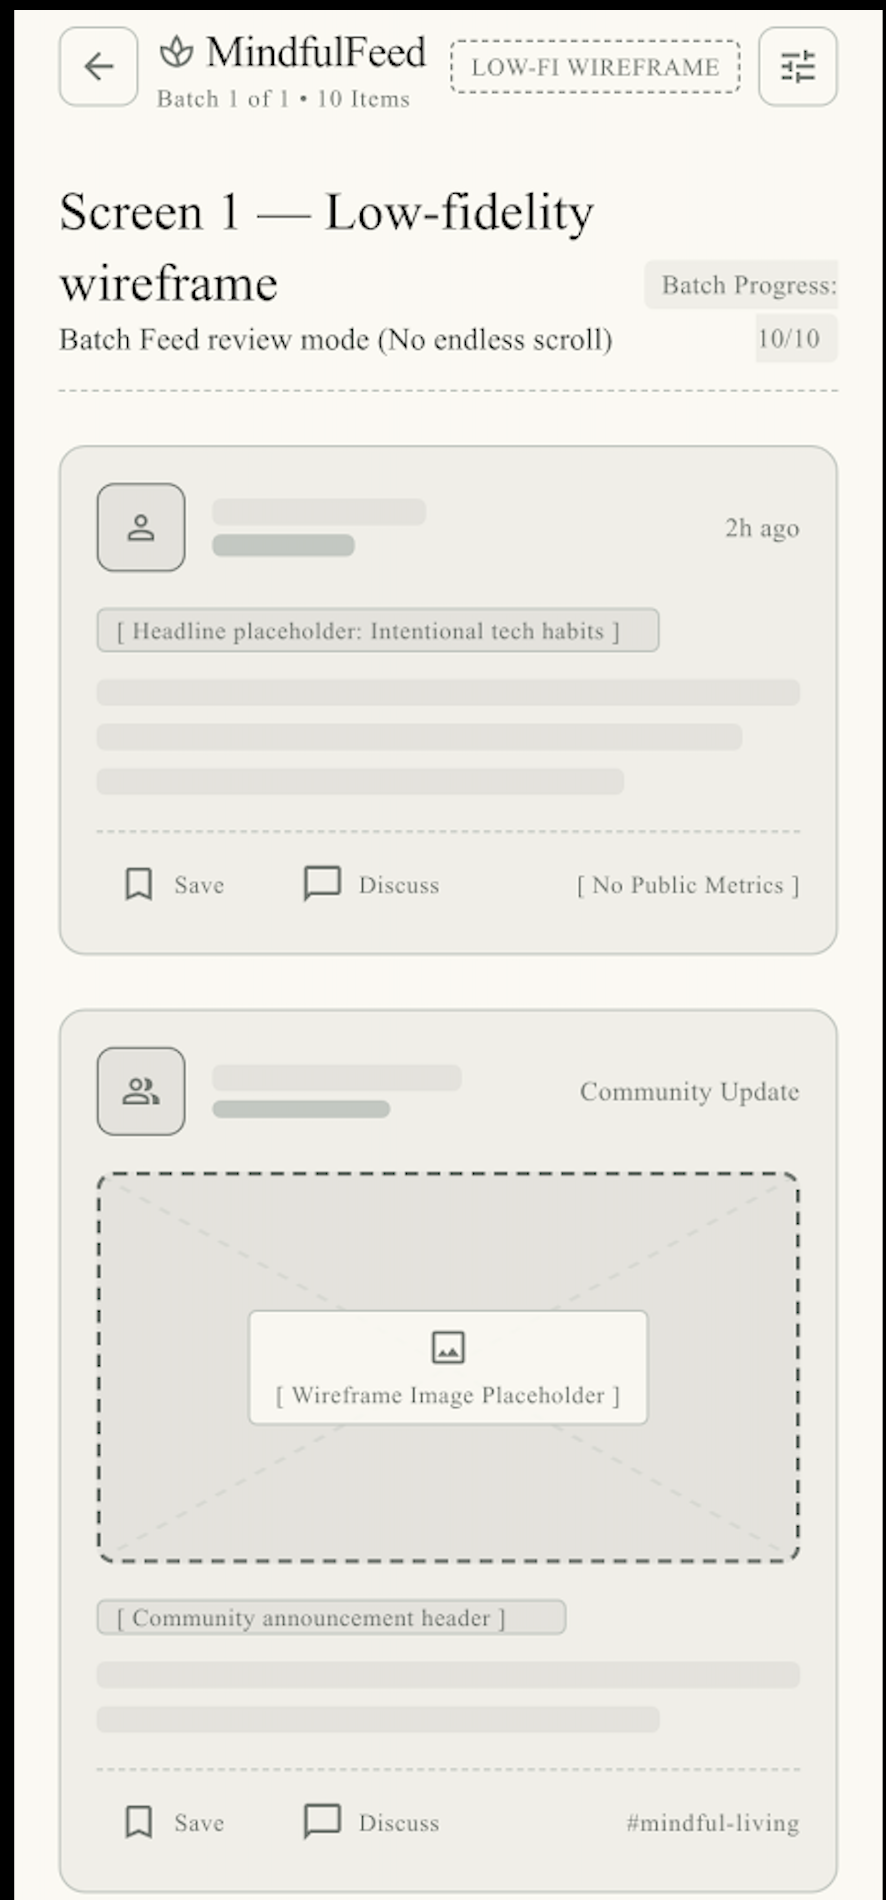
\includegraphics[width=\linewidth,keepaspectratio]{tools/images updated/Image 1 - 1.png}
\end{minipage}
\hfill
\begin{minipage}{0.47\textwidth}
\centering
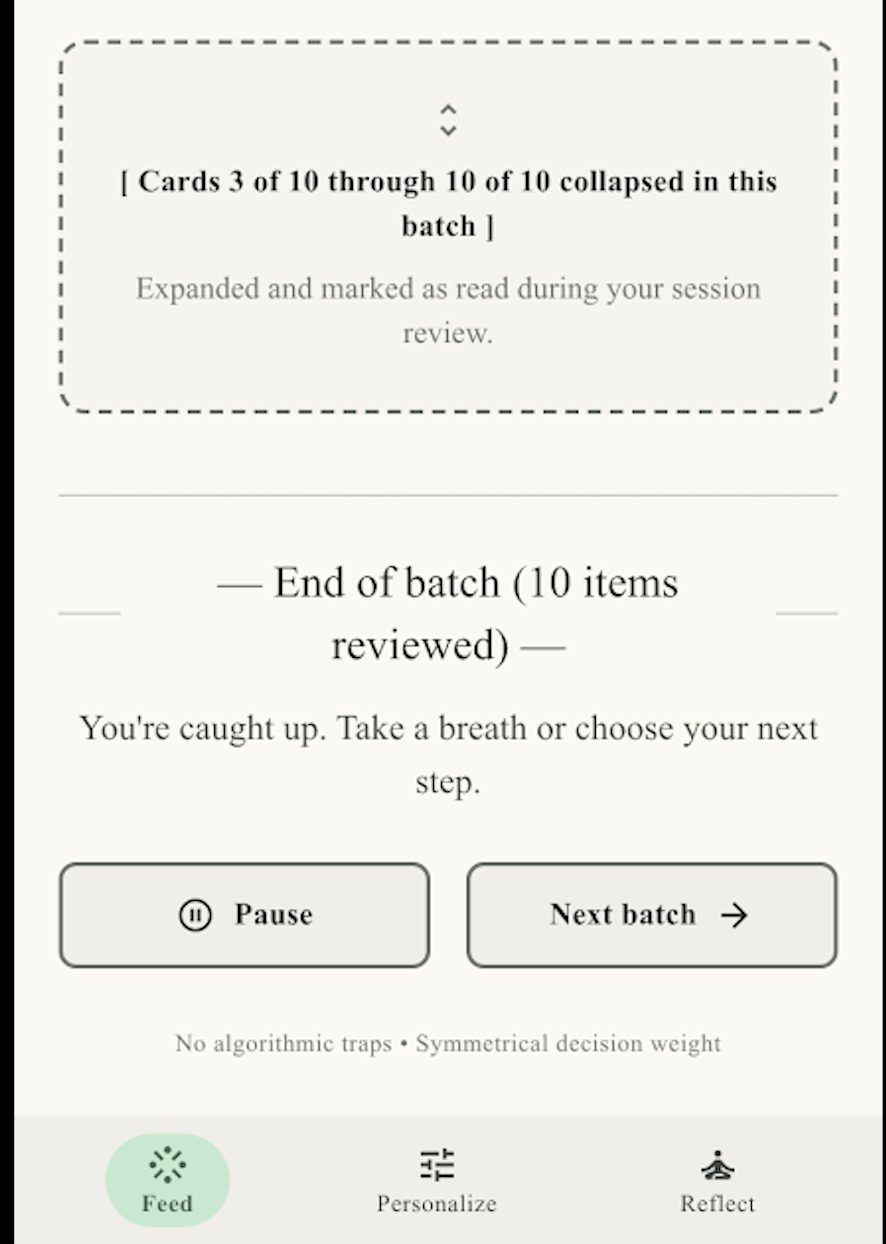
\includegraphics[width=\linewidth,keepaspectratio]{tools/images updated/Image 1 - 2.png}
\end{minipage}
\caption{Low-fidelity wireframe: batch feed with explicit end-of-batch marker (Prototype v1)}
\label{fig:wireframe_v1}
\end{figure}

Cognitive walkthroughs on v1 found that participants could complete core browsing tasks but struggled to locate opt-out controls. They read the bottom-anchored consent banner as nudging toward acceptance, matching interface-interference patterns already documented in consent-banner research \parencites[4]{4807303}[2]{5678011}. Two of the three also said the batch boundary itself felt abrupt without any explanation attached to it; one participant described it as feeling "cut off mid-thought" rather than invited to pause. The team read this as a missing-explanation problem, not a reason to abandon the stopping point itself, and carried the hard boundary forward while adding explanatory framing in v2 and v3.

\subsection{Prototype v2: Mid-Fidelity Algorithm Control Dashboard}
Prototype v2 (Figure~\ref{fig:wireframe_v2}) responded to the v1 feedback by introducing an explicit Personalization Hub with three tiers (Minimal, Balanced, Maximized) and a symmetric consent modal.

\begin{figure}[H]
\centering
\begin{minipage}{0.47\textwidth}
\centering
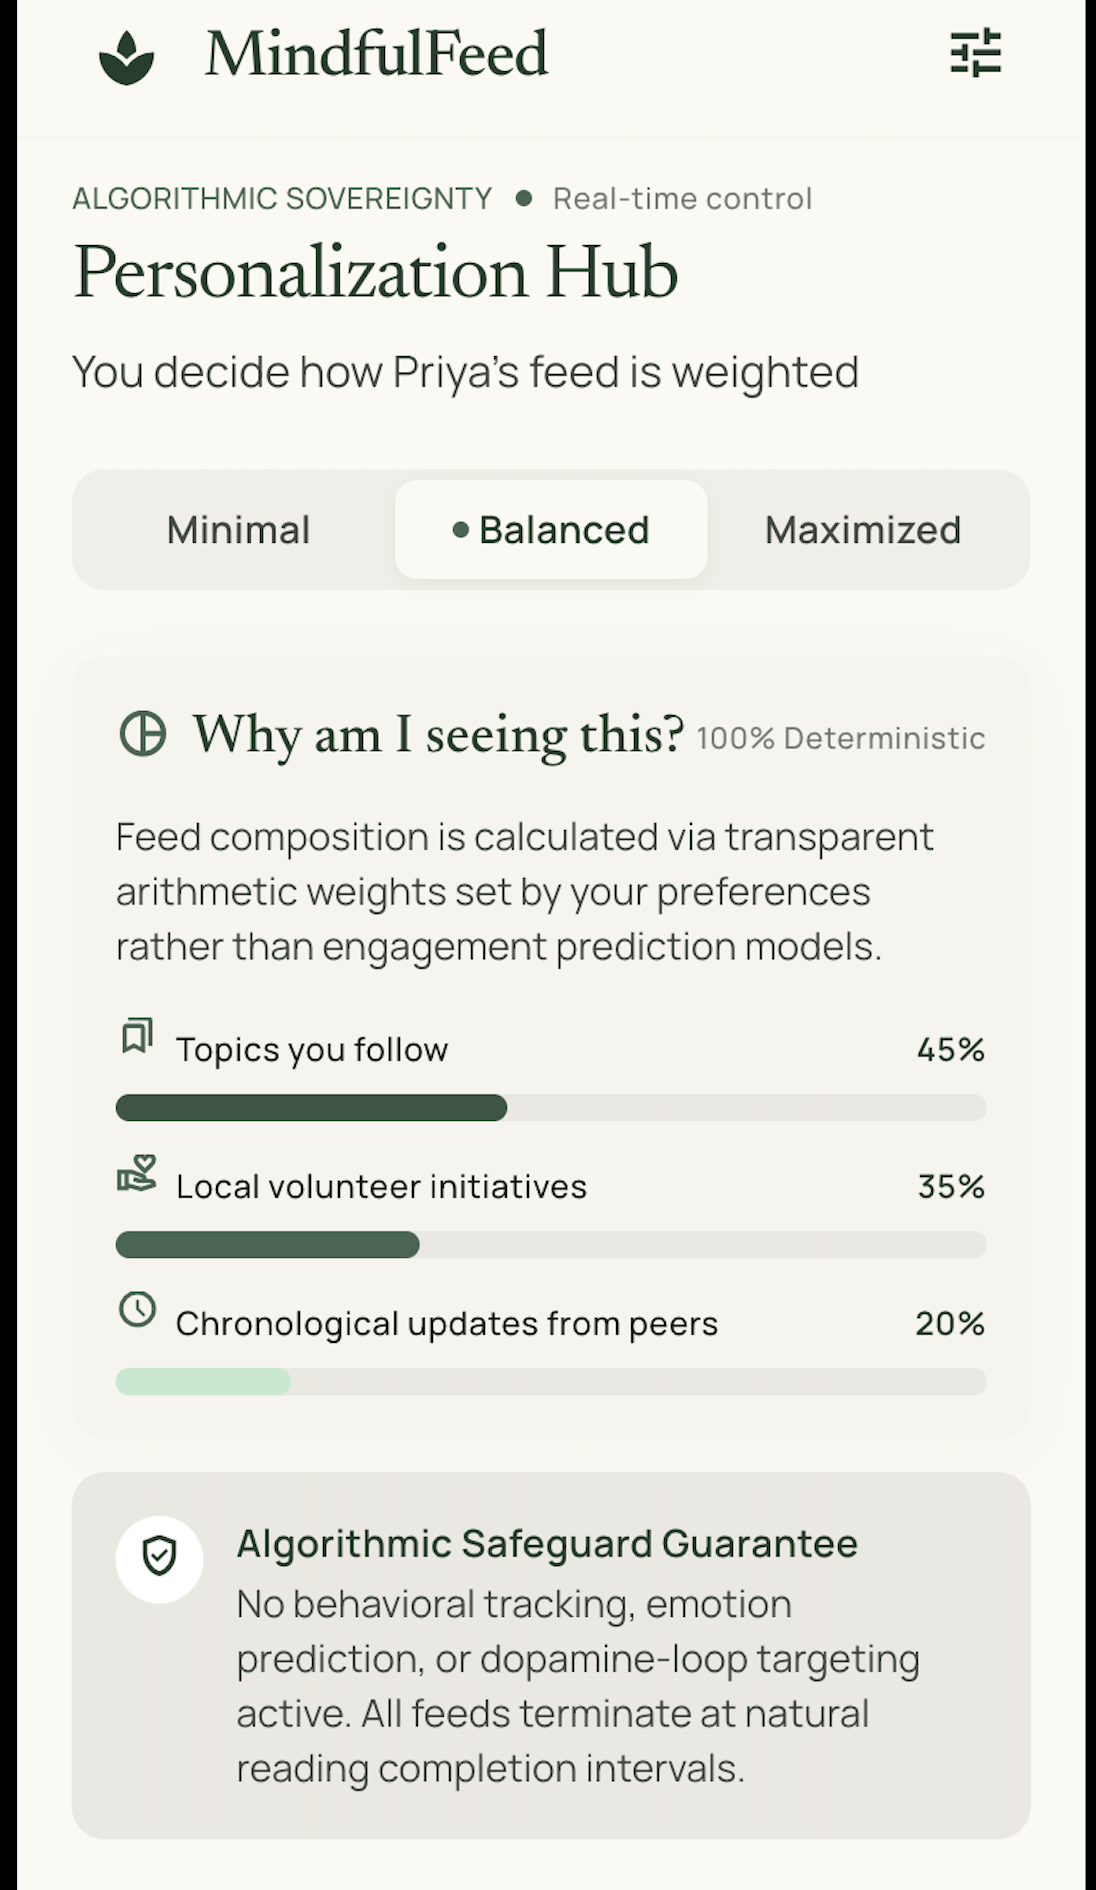
\includegraphics[width=\linewidth,keepaspectratio]{tools/images updated/Image 2 - 1.png}
\end{minipage}
\hfill
\begin{minipage}{0.47\textwidth}
\centering
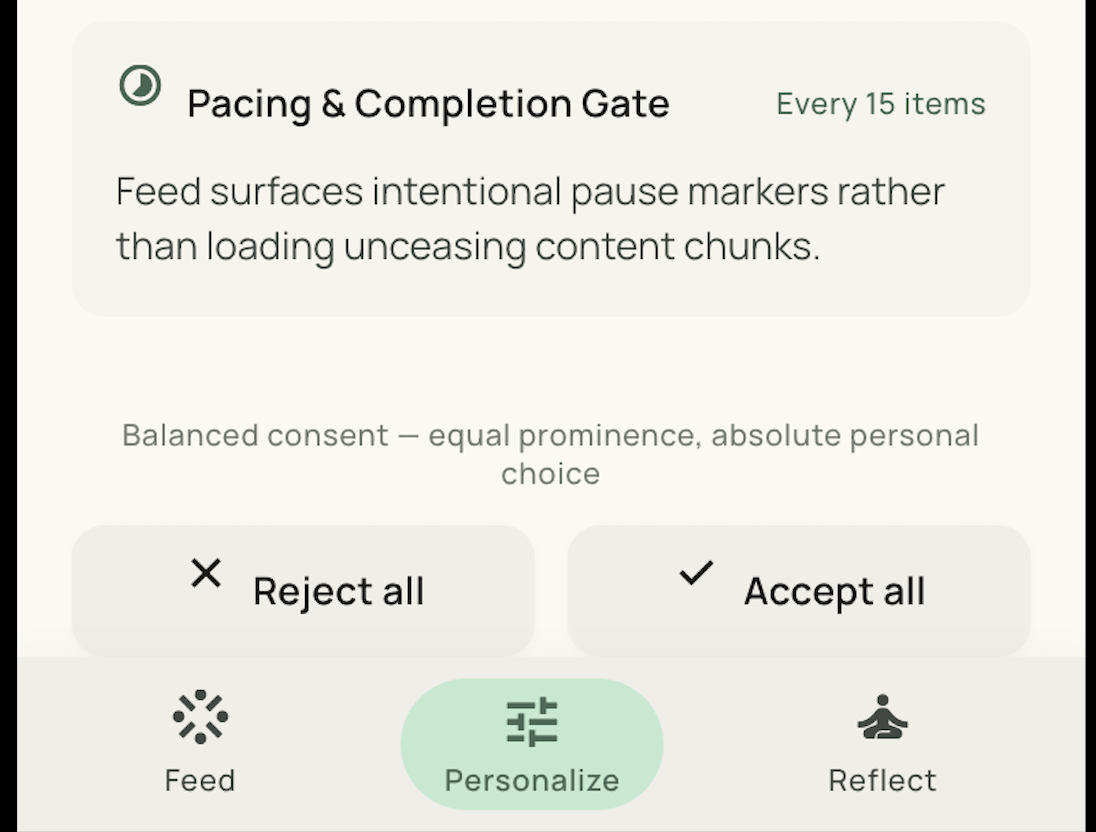
\includegraphics[width=\linewidth,keepaspectratio]{tools/images updated/Image 2 - 2.png}
\end{minipage}
\caption{Mid-fidelity wireframe: algorithm control dashboard with symmetric consent (Prototype v2)}
\label{fig:wireframe_v2}
\end{figure}

The cognitive walkthrough revealed friction with accessing the granular category-level toggle buttons that sit behind the tier select toggle, showing that navigation depth alone can reintroduce obstruction even after an obvious dark pattern has been removed \parencites[3]{4692551}. Removal of the asymmetric consent banner was not enough though, because the "turn tracking off" link at the bottom of the navigation page was still not as easily accessible as the "keep tracking on."

\subsection{Prototype v3: High-Fidelity Interactive System}
Prototype v3 (Figure~\ref{fig:wireframe_v3}) flattened the navigation flagged in v2 and added a one-click "Continue without personalization" path, a preset-mode selector, and an Ethical AI Compliance indicator. In response to the v2 feedback, the preset modes (Focus, Discovery, Social) replaced the v2 tier selector directly. Rather than asking users to reason about the abstract idea of personalisation intensity, v3 asks them to pick a familiar intent, and maps that choice internally onto the same tracking-granularity and content-diversity settings v2 exposed directly. It gives up a little technical transparency in exchange: participants configuring v2 reported real cognitive load, and none of the asymmetric defaults from the earlier prototypes came back in the trade.

\begin{figure}[H]
\centering
\begin{minipage}{0.31\textwidth}
\centering
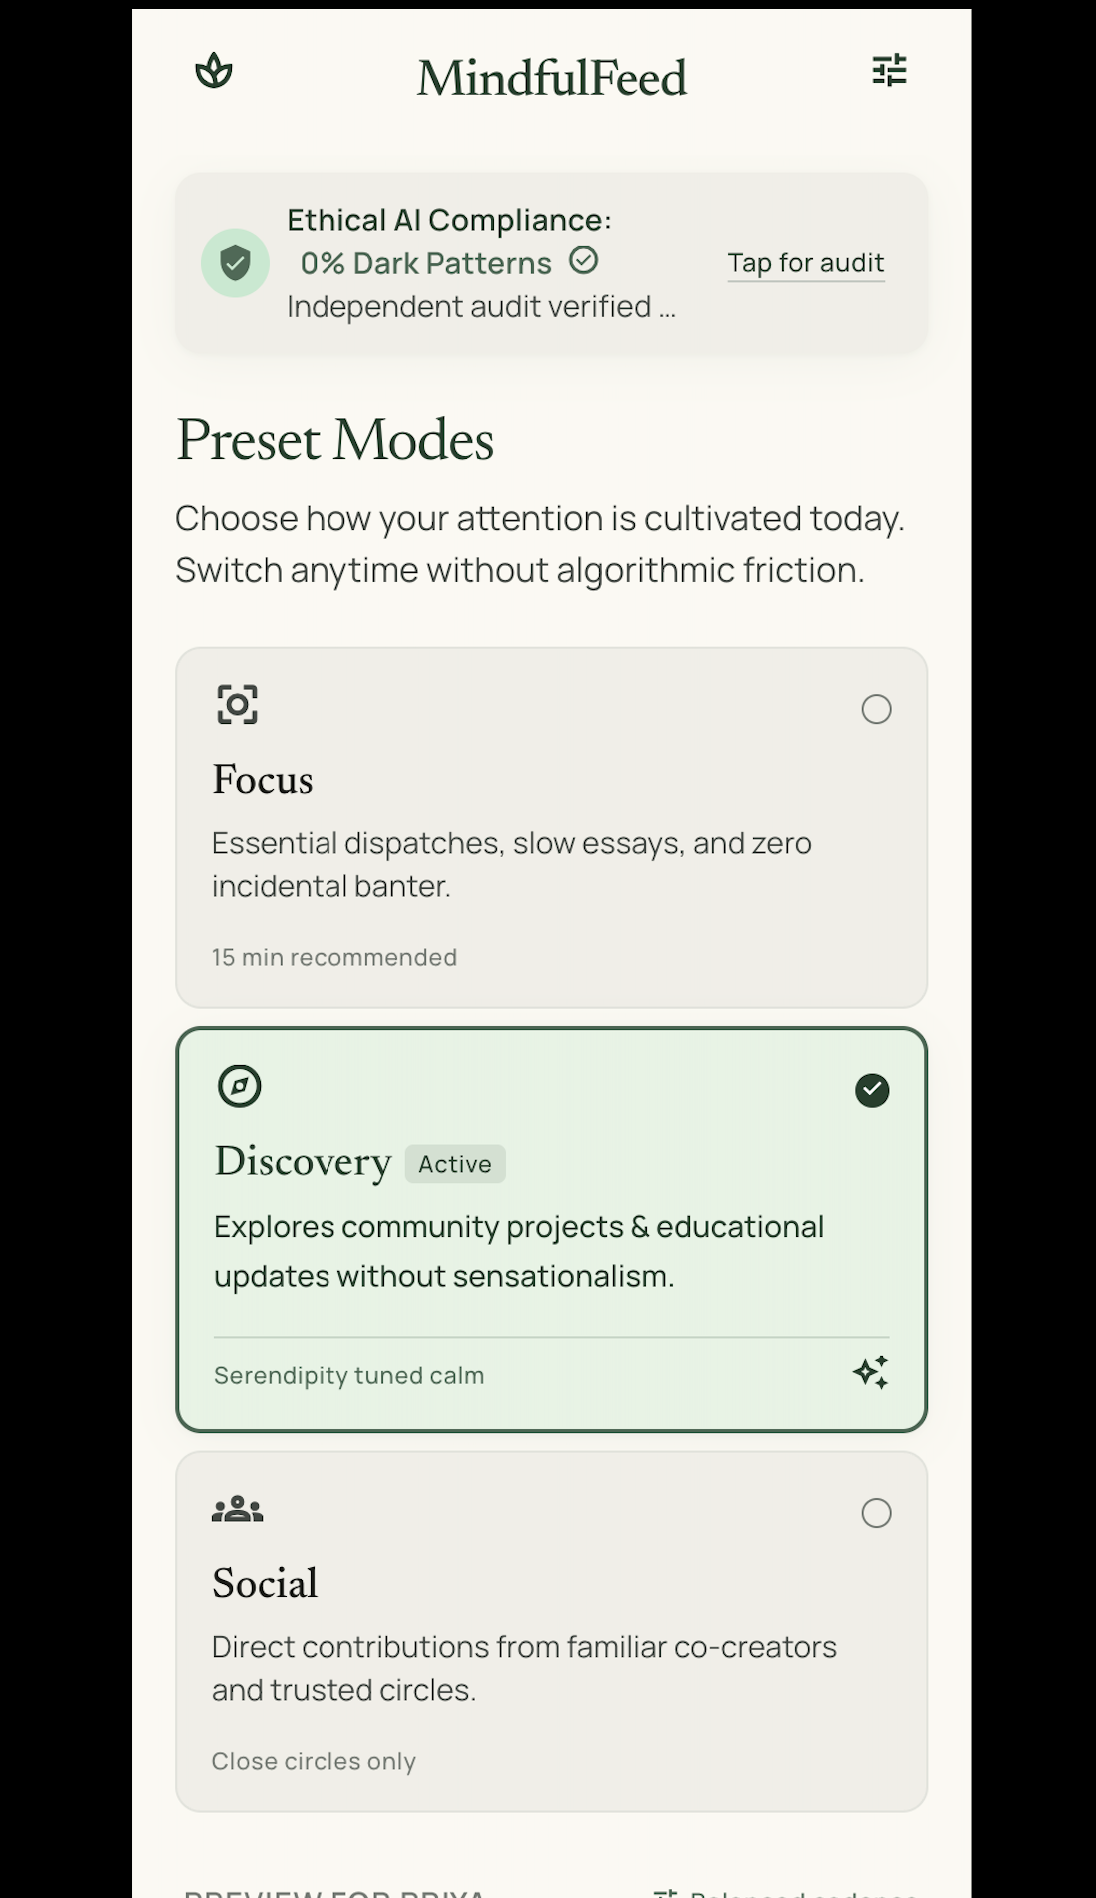
\includegraphics[width=\linewidth,keepaspectratio]{tools/images updated/Image 3 - 1.png}
\end{minipage}
\hfill
\begin{minipage}{0.31\textwidth}
\centering
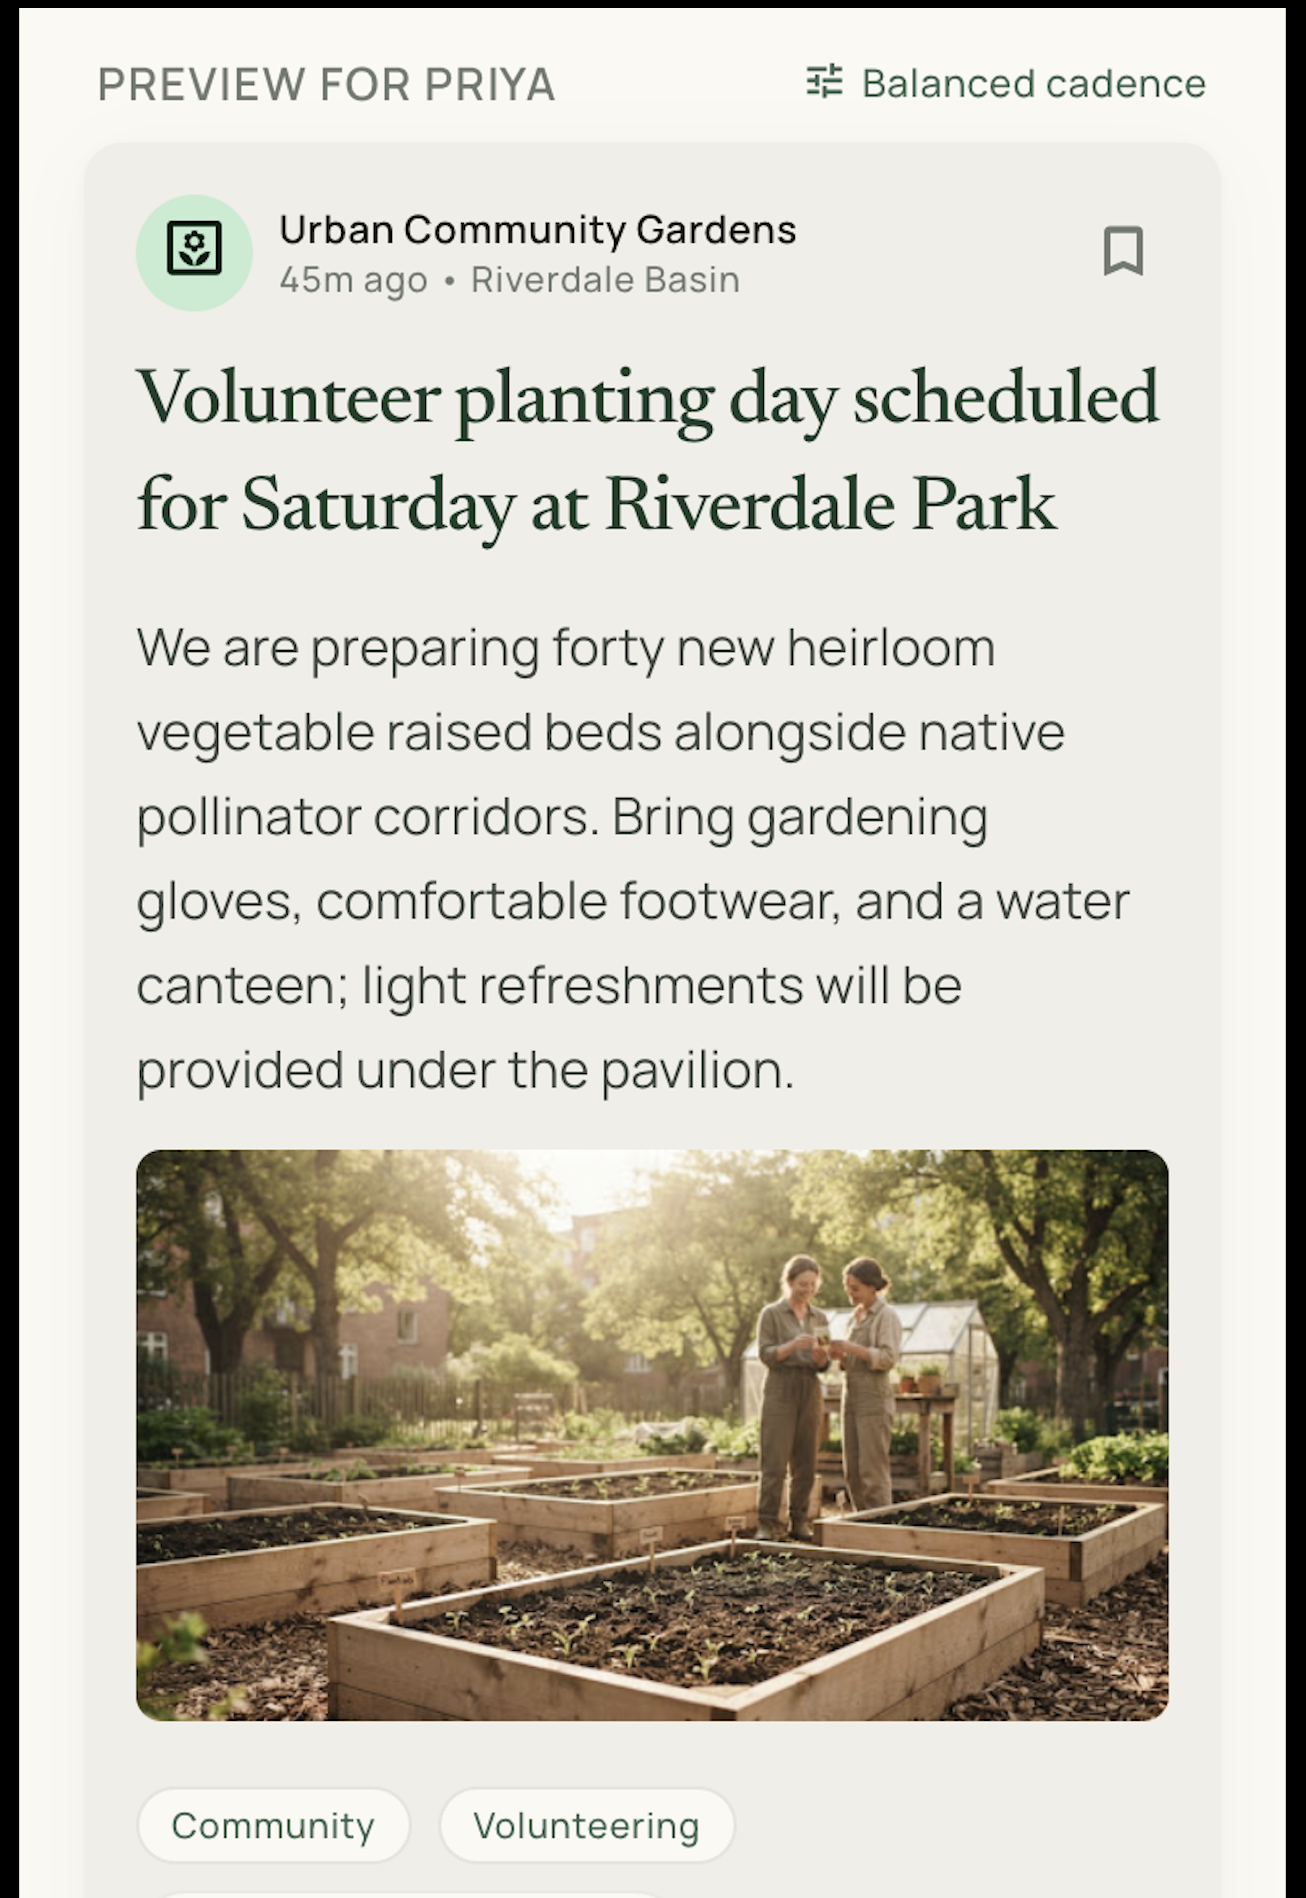
\includegraphics[width=\linewidth,keepaspectratio]{tools/images updated/Image 3 - 2.png}
\end{minipage}
\hfill
\begin{minipage}{0.31\textwidth}
\centering
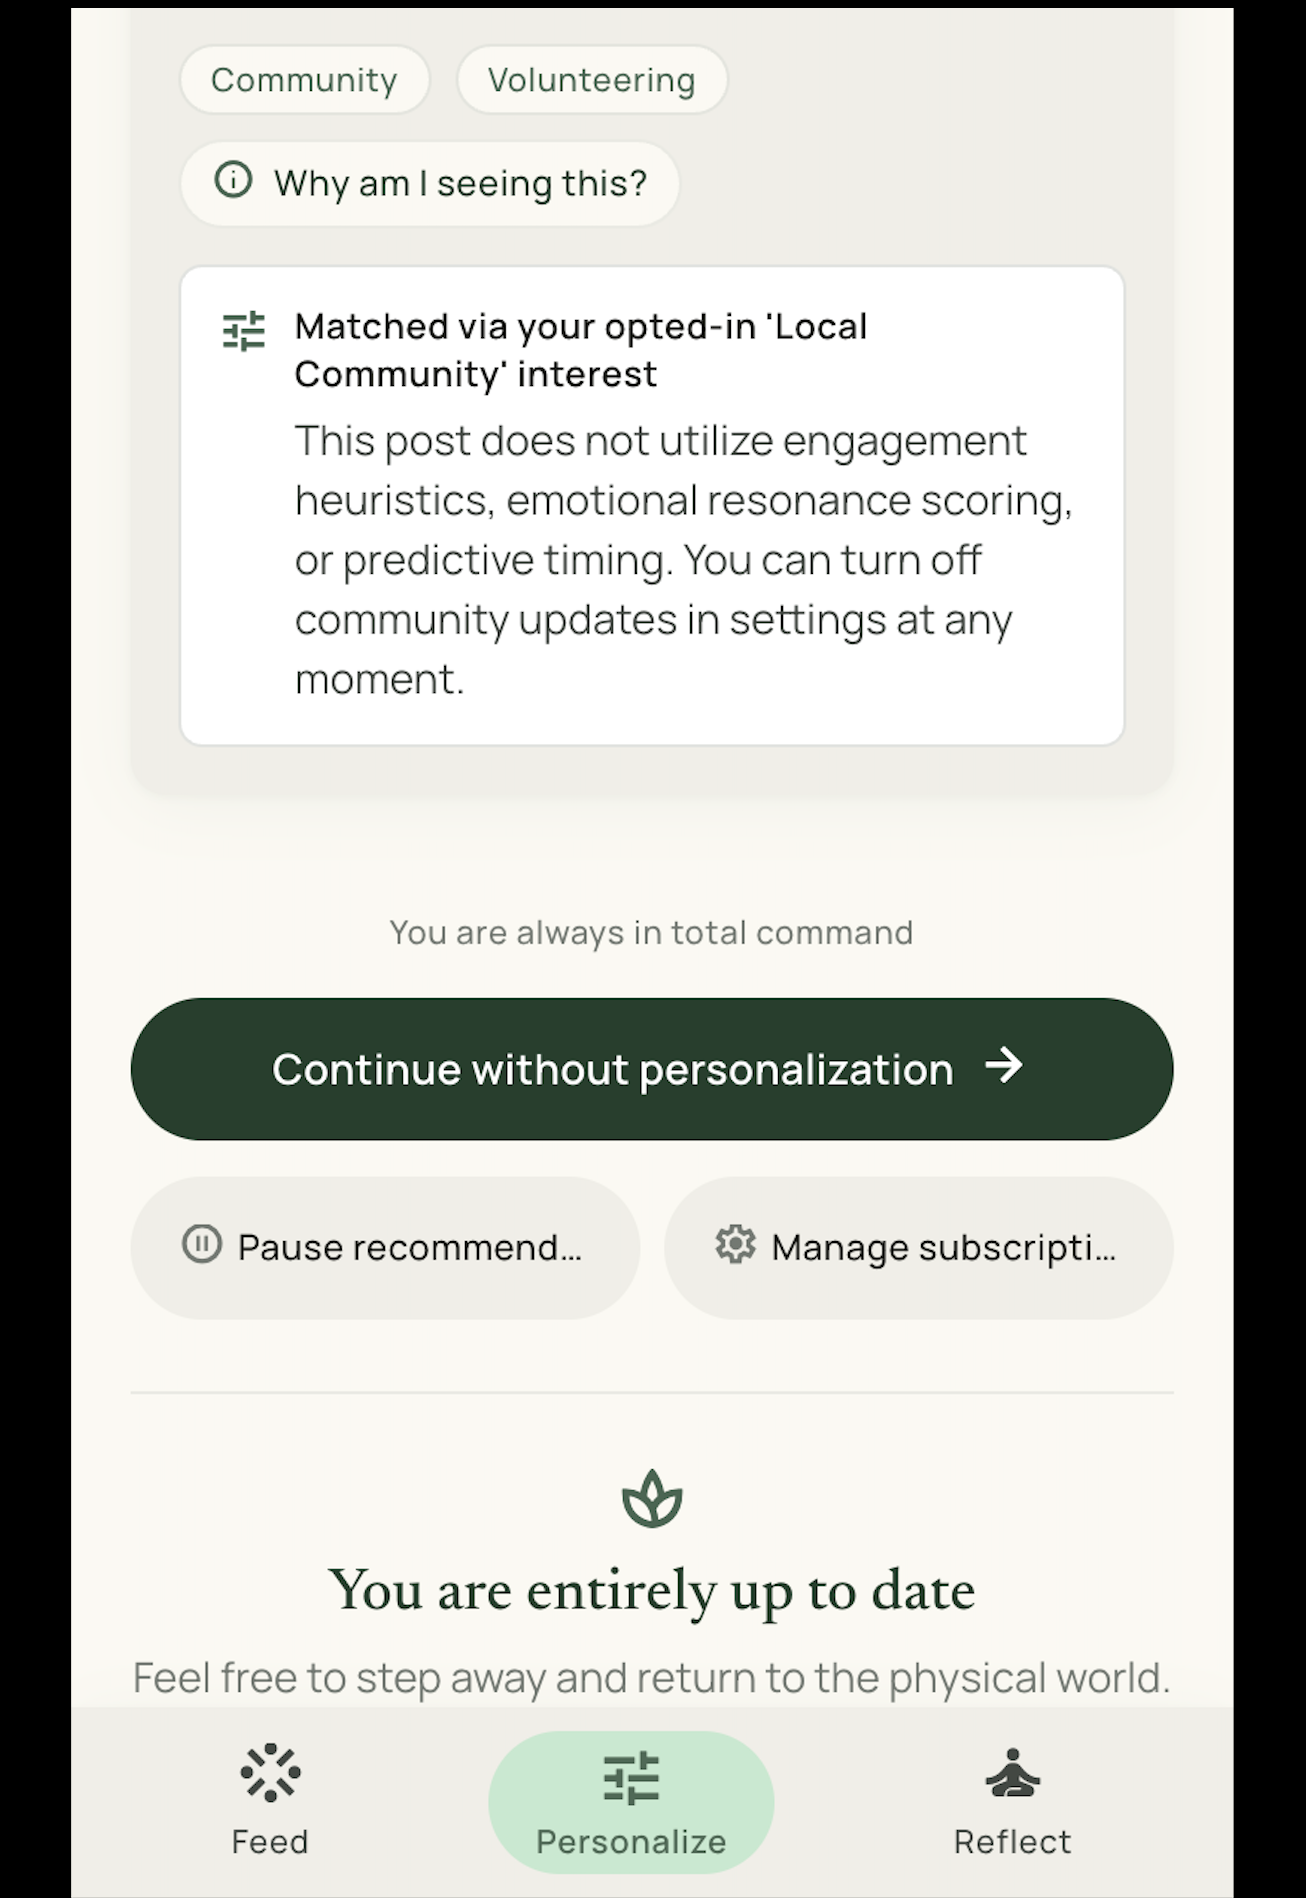
\includegraphics[width=\linewidth,keepaspectratio]{tools/images updated/Image 3 - 3.png}
\end{minipage}
\caption{High-fidelity wireframe: preset modes, compliance indicator, and symmetric refusal path (Prototype v3)}
\label{fig:wireframe_v3}
\end{figure}

\subsection{Feedback and Redesign Summary}
Table~\ref{tab:feedback_redesign_summary} traces the design decisions, feedback, identified dark-pattern risks, and redesign actions across the three prototype iterations.

% ============================================================
% 6. EVALUATION / REFLECTION
% ============================================================
\section{Strategic Evaluation and Reflection}

\subsection{Desirability, Feasibility, and Profitability}
Desirability evidence came directly from the Test phase. Participants using v3 reported higher perceived autonomy and control than with v1, and the walkthroughs on the final design turned up no unresolved obstruction or interface-interference, consistent with prior findings that symmetric opt-in/opt-out design measurably improves trust \parencites[2]{4807303}. The stronger evidence, though, is not any single score but the progression itself: each documented complaint, an abrupt stopping point, a confusing settings hierarchy, was answered by one specific, traceable change, not by redesigning the product wholesale between rounds.

This evidence has real limits worth stating rather than glossing over. Three participants across three short test rounds is enough to catch obvious obstruction and confirm a direction, but not enough to claim the product is desirable at any scale, or to rule out a fourth or fifth user surfacing a problem none of Sakshi, Arjun, or Meera happened to hit. The same three people also saw all three prototype versions in sequence, which introduces an obvious confound: some of the reported improvement from v1 to v3 may reflect growing familiarity with MindfulFeed's interface generally, rather than the specific redesign choices under test. A production evaluation would need fresh participants at each stage, or at minimum a control group that only ever saw v3, to separate learning effects from genuine design improvement. Neither was feasible within this project's timeline, and this is treated here as a limitation of the evidence rather than something the scores or the feedback table can quietly resolve on their own.

Five data points exist outside that confound, not two. Neil, Ashish, Omkar, Rahul, and Imen, the genuinely real participants introduced in Section~\ref{sec:mindfulfeed_interviews}, independently walked through all three prototype versions using the self-administered version of the same test questions (Section~\ref{sec:ai_disclosure_mindfulfeed}). Their reactions were not uniformly confirmatory of the v1-to-v3 progression argued above, and the clearest disagreement is not between any two individuals but a majority pattern: three of the five, Omkar, Rahul, and Imen, named v2, not v3, as the version they trusted most. Omkar's reasoning was explicit: v2 ``explicitly shows what's happening behind personalisation,'' and for him, more visible mechanism meant more felt control, exactly the trade-off v3's preset modes were designed to simplify away. Rahul gave a similar reason, that v2 was ``more open about\ldots what is being shown to me,'' while still rating v3 positively overall. Imen picked v2 on ``middle gut feeling'' alone, with no stated reason. Read together, these are not three isolated misreadings; they suggest that the preset-mode simplification in v3, adopted specifically in response to v2's cognitive-load feedback (Section~\ref{sec:prototype_test_mindfulfeed}), may have traded away enough visible mechanism to cost some users' trust even as it earned others' ease of use.

This larger picture does not erase Neil and Ashish's original disagreement. Neil read v1's top-of-screen element as an identification marker rather than a feed control, was unsure what the ``Balanced'' tier label in v2 meant, and read v3's ``0\% Dark Patterns'' banner as a statement about AI content detection rather than the product's own design commitment, then chose v1 as most trustworthy anyway, reasoning that it ``looks less like an AI slop.'' Ashish read the v2 label correctly, did not feel nudged by the consent screen, and chose v3 specifically because it was ``easiest to understand.'' Imen's walkthrough surfaces a sharper version of Neil's comprehension gap: she did not know what ``batch'' meant (``what's a batch''), had ``no idea'' what the ``0\% Dark Patterns'' banner communicated, and rejected the underlying premise outright, saying she would not use an app like this instead of a normal feed because it looked ``too bland.'' Omkar and Rahul, meanwhile, both located v2's opt-out control indirectly, through the settings menu or the ``Minimal'' tier, rather than through the tier's direct reject action, echoing the exact opt-out-discoverability problem the v1-to-v2 redesign was supposed to have fixed (Section~\ref{sec:prototype_test_mindfulfeed}). Five real, independent data points, split three ways on which prototype to trust and two ways on whether the interface vocabulary was even legible, do not overturn a conclusion built from three simulated test rounds. The evidence base built for this report was large enough to catch obvious obstruction. It was not large enough to predict that the redesign's own biggest usability win would cost some real users' trust.

This real-user evidence also puts pressure on a design bet made back in Define (Section~\ref{sec:persona_priya}): that autonomy-preserving, soft controls, symmetric consent, tiered personalisation, a pause nudge, would be enough to restore a sense of control without resorting to blunt restrictions like hard time locks, which the DFP matrix scored low on desirability partly for that reason (Section~\ref{sec:dfp_mindfulfeed}). Imen's and Ashish's empathize-phase answers, however, both reported that soft self-regulation tools had already failed them personally, and that only deleting an app outright had worked. Nothing in MindfulFeed's three prototypes was tested against that specific failure mode, since none of the wireframe walkthroughs asked participants to imagine walking away from the product entirely rather than adjusting a setting within it. This is treated here as an open question rather than a refutation of the finite-batch-feed approach: it is possible that an explicit, low-friction stopping point succeeds precisely where implicit self-discipline, muting, time limits, fails, but the evidence collected here cannot distinguish that outcome from the alternative, that Imen's and Ashish's pattern generalises and no amount of soft-control redesign moves users who have already concluded that deletion is the only tool that works.

A second limit concerns what "desirability" was actually measured against. The walkthroughs and interviews captured whether participants could locate controls and whether they reported feeling more in control, but they did not measure whether MindfulFeed's core premise, a feed with a hard stopping point, would survive sustained real-world use once the novelty of a new app wore off. Sakshi's initial reaction to the batch boundary in v1 (feeling "cut off mid-thought") suggests that even a well-explained stopping point carries some ongoing friction cost that a single test session cannot fully surface; whether that friction fades with habituation or compounds into abandonment is an empirical question this project's short prototyping cycle was not positioned to answer.

There were several challenges that limited feasibility, some of which involved a delicate balance between proving tiered personalisation and not overstepping the boundaries of user control (as in the v2 version); ultimately, the team decided to flatten the v2 tiered personalisation in v3 rather than remove user control. Another constraint fell outside the scope of this project: the recommendation engine. It is simple to show a "Why am I seeing this?" label in an interface for every feed item. Generating an accurate and understandable explanation to a non-technical user is not; that's a decision on model architecture outside of the interface prototypes developed here, and the report records it as an open requirement for a future implementation phase.

Section~\ref{sec:dfp_mindfulfeed} scored profitability on a subscription model rather than advertising. Ad-driven, engagement-maximising monetisation is the mechanism most directly implicated in the dark patterns the product exists to avoid \parencites[2]{5127387}, so building the product around it would have contradicted the design criteria set in Define. A subscription model also fits Priya better: her stated frustration was with feeling watched and used for her attention, and a subscription relationship changes what the product optimises for, renewals rather than viewer-engagement-point-maxing, without needing the same engagement-maximising mechanics the interviews flagged as harmful. Whether users will actually pay for a calmer feed is untested here, and that gap is a real financial risk, not an assumption to wave away.

\subsection{Critical Reflection on the d.School Process}
\label{sec:dschool_critical_reflection}
The five-phase structure gave the project a clear, auditable trace from interview evidence (Empathize) through to a tested design (Prototype/Test), keeping ideation tethered to documented pain points instead of speculative features. Fixing the persona and POV statement before ideation began also had a useful disciplining effect: when ideas like continuously adaptive reward schedules resurfaced in the Ideate phase, the team could reject them on the simple grounds that they did not match the persona's stated needs, without re-arguing the point every time.

The main limitation surfaced in Ideate. SCAMPER and the DFP matrix work well for interface-level concepts, but they say almost nothing about how an underlying recommendation algorithm should actually be trained or audited. The project addressed that gap only at the level of design constraints: symmetric effort, explainability, human oversight. It never touched algorithm design itself, and it would be disingenuous to claim otherwise.

A second limitation is more procedural, and only became visible in hindsight. The five-phase model treats Prototype and Test as one combined stage. This project ran three short cycles instead, build, test, redesign, three times over, not one long prototyping phase followed by a single test. The upside was real: three separate rounds of feedback produced more, smaller redesign decisions than one big round would have. The cost showed up later, in the Evaluation section above: it became harder to say cleanly whether a given improvement in v3 came from the preset-mode change, the flattened navigation, or the two acting together. A cleaner experimental design would have changed one variable at a time between prototypes. This project changed several at once in both the v1-to-v2 and v2-to-v3 transitions, trading causal clarity for development speed, a trade the team would make differently with more time available.

% ============================================================
% 7. CONCLUSION
% ============================================================
\section{Conclusion}

\subsection{Synthesis of Results}
This project report traced MindfulFeed's design thinking process from three empathize-phase interviews through a synthesised persona, a point-of-view statement, four How-Might-We questions, SCAMPER-generated concepts filtered through a DFP matrix, and three progressively tested prototypes. Each phase produced one specific, traceable artefact instead of a general discussion of the problem space. Every design change in the Prototype/Test cycle traces back to a documented piece of feedback, not an assumption: the move from an implicit slider (v1) to explicit tiers (v2) to preset modes (v3) is attributable to the specific usability findings recorded in Table~\ref{tab:feedback_redesign_summary}, and nothing in that progression was left to unstructured iteration.

The resulting product record shows a feasible path from documented user harm, compulsive engagement, algorithmic opacity, conflict-driven exhaustion, to a concrete, testable interface response: batch feeds, tiered personalisation, symmetric consent, and non-manipulative monetisation. The persona synthesis in Section~\ref{sec:persona_priya} also makes a smaller point worth stating plainly: one evidence-based persona can absorb design-relevant detail from more interview participants than it literally represents, as long as the synthesis step is written down rather than left implicit.

\subsection{Critical Reflection on Methodology}
Section~\ref{sec:dschool_critical_reflection} already set out where the d.School model earned its keep, an auditable trace from interview evidence to a tested design, and where it did not: the DFP matrix has almost nothing to say with regard to the actual training and auditing of any underlying recommendation algorithm. That limitation carries directly into what remains open for future work. This project addressed the algorithmic-governance gap only as a design constraint, symmetric effort, explainability, human oversight, not as an algorithm specification, and treating those interface-level constraints as a substitute for governing the model itself would overstate what a five-phase design thinking process alone can settle.

\subsection{Outlook for Future Practice}
Section~\ref{sec:context_motivation} noted that a designer using a dark pattern ten years ago risked a bad blog post, while today the same choice risks a regulatory finding under the Digital Services Act, with the anticipated EU Digital Fairness Act (Q4 2026) expected to restrict manipulative interfaces directly. MindfulFeed's core controls, symmetric opt-in/opt-out consent, explainable personalisation tiers, a one-click refusal path, were built to the DFP matrix's desirability and feasibility scores, not to a specific regulatory clause. That they also happen to anticipate what the DFA is expected to require is worth stating plainly: the practical shift this project points to is that ethical interface design is moving from a marketing differentiator, a way to stand out, toward a compliance baseline that platforms operating in the EU will need regardless of whether they choose to advertise it. Whether MindfulFeed's specific mechanisms, batch feeds, tiered consent, would satisfy an eventual DFA audit is untested here; what this report can support is narrower: that building those mechanisms from documented user evidence, rather than from the letter of an anticipated regulation, is itself a defensible starting point for that transition.

\clearpage
\printbibliography

\clearpage
\appendix
\section{Appendix: Supporting Tables}
\label{sec:appendix_tables}
This appendix collects the tables referenced throughout the design thinking narrative in Sections 1--5: the framework comparison, the interview and empathy-map artefacts, the persona summary, and the ideation and prototyping matrices. Each table is discussed at the point in the main text where it is cited.

\begin{table}[H]
\centering
\caption{Comparison of candidate design thinking frameworks}
\label{tab:framework_comparison}
\small
\begin{tabular}{p{3cm}p{6cm}p{6cm}}
\hline
\textbf{Framework} & \textbf{Structure} & \textbf{Rationale} \\
\hline
Stanford d.School (\textbf{selected}) & Empathize, Define, Ideate, Prototype, Test & Distinct Define phase separates problem framing from ideation, and the explicit Prototype/Test split matches the project's need for three traceable, independently tested design iterations. \\
IDEO Field Guide to Human-Centered Design & Inspiration, Ideation, Implementation & Rejected: collapses problem definition into Inspiration, giving less structure for documenting a discrete persona and POV statement ahead of ideation. \\
HPI Micro-Cycle & Understand, Observe, Synthesise, Ideate, Prototype, Test & Rejected: the Understand/Observe/Synthesise split is largely redundant for a software interface project where empathize-stage interviews already combine observation and synthesis. \\
\hline
\end{tabular}
\end{table}

\begin{table}[H]
\centering
\caption{MindfulFeed interviewee profiles and burnout triggers}
\label{tab:profiles_mindfulfeed}
\small
\begin{tabular}{p{1.8cm}p{2.6cm}p{3.2cm}p{3.2cm}p{5.5cm}}
\hline
\textbf{Name} & \textbf{Role} & \textbf{Goals with MindfulFeed} & \textbf{Burnout Triggers} & \textbf{Representative Quote} \\
\hline
Sakshi & Undergraduate student & Stay socially updated between study sessions & Late-night personalised recommendations, fear of missing out, sleep-disrupting notification loops & \textit{"I open MindfulFeed for five minutes before bed and suddenly it is two hours later."} \\
Arjun & Marketing professional & Monitor trends and manage brand channels efficiently & Overlapping work/personal feeds, pressure to respond instantly & \textit{"My job is inside MindfulFeed, but sometimes it feels like I can never log off."} \\
Meera & Community organiser & Coordinate events and advocacy content & Repetitive suggested debates, emotional drain from conflict threads & \textit{"I come here to support causes, but the arguments follow me everywhere."} \\
Neil\textsuperscript{*} & Tech support specialist & Quick entertainment and social check-ins between work tasks & Reflexive hour-plus binges on football and meme content; harmful content surfacing unprompted & \textit{"Antisemitism."} (his answer, unprompted, when asked what frustrates him most about his feed) \\
Ashish\textsuperscript{*} & Software engineer & Kill short gaps in the day; open, scroll briefly, close & Low tolerance for irrelevant content; self-regulates by using mobile web instead of the app & \textit{"Boring and simply not useful."} (his answer when asked what frustrates him most about his feed) \\
Omkar\textsuperscript{*} & Engineer & Occasional relaxation browsing, without deep investment & Frustrated by over-personalisation narrowing content diversity rather than by compulsive overuse; already deleted every app except one & \textit{"Too much personalisation which shows similar stuff."} (his answer when asked what frustrates him most about his feed) \\
Rahul\textsuperscript{*} & Product manager & Stay updated and connected with friends and colleagues & Algorithmic drift from intentional friend updates into engaging-but-low-value video content; conscious of losing 15--20 minutes at a time & \textit{"You end up watching the content that has no significance (but is just engaging) \& a lot of such content."} (his answer when asked what frustrates him most about his feed) \\
Imen\textsuperscript{*} & Not disclosed (self-described only as ``im just a girl'') & Reduce compulsive doom-scrolling and ad exposure & Repeated failed attempts at muting or limiting use; only deleting the app itself changed behaviour & \textit{"ads"} (her answer when asked what frustrates her most about her feed) \\
\hline
\end{tabular}
\end{table}

\begin{table}[H]
\centering
\caption{Empathy map synthesised from the three MindfulFeed interviews}
\label{tab:empathy_map_mindfulfeed}
\small
\begin{tabular}{p{4cm} p{4cm} p{4cm} p{4cm}}
\hline
\textbf{Says} & \textbf{Thinks} & \textbf{Does} & \textbf{Feels} \\
\hline
``My feed makes me feel worse about myself after scrolling.'' & Worries that everyone else is doing better online. & Scrolls for long periods at night despite intending to stop. & Insecure about status and appearance. \\
``Recommendations are repetitive and pushy, not really for me.'' & Believes the algorithm prioritises profit over well-being. & Dismisses personalised widgets faster over time. & Fatigued by being tracked and targeted. \\
``I keep checking notifications even when I should be studying.'' & Fears missing something important if offline. & Checks the phone during study or family time. & Anxious, mentally drained, guilty about lost time. \\
``I do not fully trust platforms with my data or pricing.'' & Suspects data is tracked and pricing is opaque. & Clears cookies or switches devices to regain control. & Distrustful, feels a loss of autonomy. \\
\hline
\end{tabular}
\end{table}

\begin{table}[H]
\centering
\caption{Define phase persona: Priya}
\label{tab:persona_priya}
\small
\begin{tabular}{p{4cm}p{9.5cm}}
\hline
\textbf{Field} & \textbf{Description} \\
\hline
Age & 24 years \\
Occupation & Marketing coordinator with part-time community volunteering \\
Tech usage pattern & Checks feeds throughout the workday and again late at night; several hours of daily use across professional and personal accounts \\
Goals for using MindfulFeed & Stay informed and professionally connected while protecting sleep, focus, and emotional bandwidth \\
Frustrations with current social media & Notification overload spanning work and personal life, algorithmic opacity, comparison-induced anxiety, emotionally draining recommended debates, algorithmic drift into low-value engaging content (especially video), and over-personalisation that narrows content diversity even once understood \\
Needs from an ethical feed & Clear explanations for why content is shown, low-friction controls over personalisation intensity and diversity, content that does not amplify conflict or comparison, and a stopping point calibrated to her own habits rather than a single fixed threshold, since soft self-regulation tools have not reliably worked for her before \\
\hline
\end{tabular}
\end{table}

\begin{table}[H]
\centering
\caption{SCAMPER ideation for MindfulFeed feed features}
\label{tab:scamper_mindfulfeed}
\small
\begin{tabular}{p{2.8cm}p{11.5cm}}
\hline
\textbf{Move} & \textbf{MindfulFeed application} \\
\hline
Substitute & Replace infinite scroll with paged sessions and an explicit "Next batch" control to restore stopping cues. \\
Combine & Combine diversity-enriched recommendations with fatigue-aware nudges that prompt a pause when over-engagement signals appear. \\
Adapt & Adapt mindfulness-app break reminders into periodic reflection prompts before continuing to the next batch. \\
Modify & Replace public engagement counters with a private, optional well-being check-in. \\
Put to another use & Use emotional-signal detection to surface calmer content instead of amplifying detected outrage or arousal. \\
Eliminate & Eliminate autoplay for video and default push notifications tied to reactive engagement metrics. \\
Reverse & Reverse ranking logic from most-engaging-first to most-balanced-first, prioritising diversity over predicted click probability. \\
\hline
\end{tabular}
\end{table}

\begin{table}[H]
\centering
\caption{Desirability-Feasibility-Profitability matrix for MindfulFeed concepts}
\label{tab:dfp_mindfulfeed}
\small
\begin{tabular}{p{5.5cm}ccc}
\hline
\textbf{Concept} & \textbf{Desirability} & \textbf{Feasibility} & \textbf{Profitability} \\
\hline
Finite batch feed with stopping cues & 4 & 4 & 3 \\
Algorithm control dashboard (tiered personalisation) & 4 & 3 & 4 \\
Intentional friction / fatigue-aware pause nudges & 3 & 4 & 2 \\
Total ad prohibition & 3 & 3 & 3 \\
Hard time locks & 2 & 4 & 2 \\
\hline
\end{tabular}
\end{table}

\begin{table}[H]
\centering
\caption{Feedback and redesign summary for MindfulFeed prototypes}
\label{tab:feedback_redesign_summary}
\small
\begin{tabular}{p{1.3cm}p{2.8cm}p{2.8cm}p{2.8cm}p{2.8cm}}
\hline
\textbf{Version} & \textbf{Key decisions} & \textbf{Feedback} & \textbf{Dark pattern risk} & \textbf{Redesign action} \\
\hline
v1 & Single inline consent banner; implicit personalisation slider; default high personalisation. & Users completed tasks but could not find opt-out; the cognitive walkthrough flagged a low-salience rejection option. & Interface interference via highlighted accept; default bias from preselected high personalisation. & Elevate consent to a modal with symmetric actions; add explicit tiers. \\
v2 & Three-tier Personalization Hub; modal consent with equal-weight Accept/Reject. & Improved perceived control; some fatigue reaching granular toggles. & Emerging obstruction from deep-nested advanced options. & Flatten navigation; add a single-screen settings overview. \\
v3 & One-click refusal path; preset modes; Ethical AI Compliance indicator; pause toggle. & Higher perceived autonomy; residual concern about long-term data retention clarity. & Reduced interference and obstruction; residual misdirection risk if future features compete for attention. & Lock symmetric flows as a design constraint; add retention-horizon indicators. \\
\hline
\end{tabular}
\end{table}


\clearpage
\section{Appendix: Supporting Figures}
\label{sec:appendix_figures}
This appendix collects the project timeline referenced in Section 1. The three prototype wireframes (v1--v3) appear inline in Section 5, at the point in the main text where each is discussed.

\begin{figure}[H]
\centering
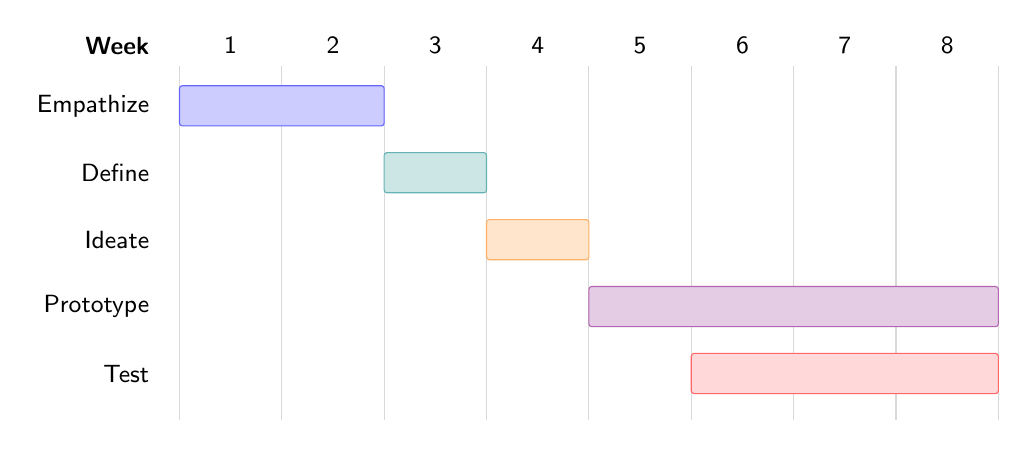
\begin{tikzpicture}[x=1.3cm, y=0.85cm]
  \foreach \w in {0,...,8} {
    \draw[gray!30] (\w,0.3) -- (\w,-5.0);
  }
  \foreach \w in {1,...,8} {
    \node[font=\small] at (\w-0.5,0.6) {\w};
  }
  \node[font=\small\bfseries, anchor=east] at (-0.2,0.6) {Week};

  \node[font=\small, anchor=east] at (-0.2,-0.3) {Empathize};
  \draw[fill=blue!20, draw=blue!60, rounded corners=1pt] (0,-0.6) rectangle (2,0);

  \node[font=\small, anchor=east] at (-0.2,-1.3) {Define};
  \draw[fill=teal!20, draw=teal!60, rounded corners=1pt] (2,-1.6) rectangle (3,-1);

  \node[font=\small, anchor=east] at (-0.2,-2.3) {Ideate};
  \draw[fill=orange!20, draw=orange!60, rounded corners=1pt] (3,-2.6) rectangle (4,-2);

  \node[font=\small, anchor=east] at (-0.2,-3.3) {Prototype};
  \draw[fill=violet!20, draw=violet!60, rounded corners=1pt] (4,-3.6) rectangle (8,-3);

  \node[font=\small, anchor=east] at (-0.2,-4.3) {Test};
  \draw[fill=red!15, draw=red!60, rounded corners=1pt] (5,-4.6) rectangle (8,-4);
\end{tikzpicture}
\caption{Project execution timeline across the five d.School phases}
\label{fig:timeline}
\end{figure}

\clearpage
\section{Appendix: GenAI Usage Disclosure}
\label{sec:ai_disclosure_mindfulfeed}
Generative AI tools were used in this project in three specific, bounded ways, disclosed here in line with the university's plagiarism and AI-use guidelines.

\begin{enumerate}
\item \textbf{Simulating interview quotes and empathy-map synthesis (Section~\ref{sec:mindfulfeed_interviews} and Section~\ref{sec:empathy_map_mindfulfeed}).} Because recruiting and interviewing real participants was outside the scope achievable for this exercise, the three interview profiles (Sakshi, Arjun, Meera) and their quoted statements were generated with AI assistance to simulate plausible qualitative feedback across three distinct usage contexts (student, working professional, community organiser). Example prompt used: \textit{"Re-enact a semi-structured interview excerpt from a [role] describing frustration with [specific dark pattern], in their own words, including one verbatim-style quote and the emotional impact reported."} Rationale: the assignment brief explicitly permits GenAI-simulated qualitative user data provided it is disclosed and combined with genuine design judgement, which the project team applied in selecting which simulated themes to retain and how to code them into the empathy map. To satisfy the further requirement that real users be used \textit{in conjunction with} AI-generated data, five genuinely real participants (Neil, Ashish, Omkar, Rahul, and Imen, Section~\ref{sec:mindfulfeed_interviews}) were separately recruited and answered the same interview questions, plus a full walkthrough of all three prototype versions (Section~\ref{sec:prototype_test_mindfulfeed}), using a self-administered testing tool built for this purpose (a single-file, offline web page; no external dependencies, no data transmitted anywhere). Their answers were typed directly by them, recorded verbatim with an automatically logged response time per question, and are reported unedited, including where they contradict the simulated evidence or each other. AI assistance was used to draft the tool's question wording, adapting the wireframe-walkthrough questions from a pre-existing human-authored testing protocol and independently drafting the empathize-interview question set from the same structure described in Section~\ref{sec:mindfulfeed_interviews}; AI was not used to generate or alter any of the five real participants' answers.
\item \textbf{Language editing.} Phrasing improvements and grammar/style consistency checks in drafted sections were suggested using AI tools. All factual and citation content was written, sourced, and verified by the author against the original literature; AI was not used to generate citations, select sources, or produce the SCAMPER, DFP, or feedback/redesign table content, which reflect the author's own design judgement.
\item \textbf{Prototype mockup generation (Section~\ref{sec:prototype_test_mindfulfeed}, Figures~\ref{fig:wireframe_v1}--\ref{fig:wireframe_v3}).} The three prototype visuals were produced with an AI UI-generation tool (Google Stitch), prompted with the specific screen contents and interaction elements the project team had already specified from the DFP-selected concepts and the v1/v2/v3 feedback progression (e.g., the batch-feed structure, the three-tier Personalization Hub, the preset-mode selector and compliance indicator). The tool rendered the visual layout; the underlying design decisions, control names, information architecture, and the redesign logic between versions were determined by the project team based on the cognitive-walkthrough findings reported in Section~\ref{sec:prototype_test_mindfulfeed}, not generated by the tool.
\end{enumerate}

No AI tool was used to generate the reference list or any numerical scoring in the DFP matrix.

\clearpage
\section{Appendix: Real-User Testing Tool}
\label{sec:testing_tool_appendix}
To collect the five real participant responses reported in Section~\ref{sec:mindfulfeed_interviews} and Section~\ref{sec:prototype_test_mindfulfeed}, the project team built a small, self-administered testing tool rather than relying on manually facilitated sessions. This appendix documents its strategy, question quality, target, and hosting, as evidence of how the requirement to use real users in conjunction with AI-generated data (Section~\ref{sec:ai_disclosure_mindfulfeed}) was actually put into practice, not only claimed.

\subsection{Strategy}
The tool ran a single combined session per participant, covering both evidence needs in one sitting rather than two separate recruitment rounds: eight prototype-walkthrough questions (Part 1), followed by eight empathize-style habit questions (Part 2), taking roughly ten to fifteen minutes end to end. Participants received only a minimal framing before starting, that they would react to three versions of an app screen and then answer general habit questions, with no explanation of the underlying design rationale, the DFP scoring, or what answer the team expected to hear. This followed the same logic as the pre-existing human-authored testing protocol the wireframe questions were adapted from (Section~\ref{sec:ai_disclosure_mindfulfeed}, item 1): unprompted, first-impression reactions were treated as more diagnostic than reactions collected after the product had already been explained.

\subsection{Questionnaire Quality}
Each of the sixteen questions was shown one at a time, with its relevant wireframe image attached where applicable, and the tool recorded the exact time between a question appearing and an answer being submitted. That per-question response-time log turned out to matter: Rahul's 750-second response to the first wireframe question and Imen's 14-second response to the same question are themselves evidence of how differently two real participants engaged with an identical prompt, a signal a plain transcript would not have captured. Participants supplied a one-line self-description (e.g., "29, swe, has no time") instead of a full demographic form, keeping the tool quick to complete without discarding the profile context needed for Table~\ref{tab:profiles_mindfulfeed}. Answers were free-text and unconstrained, entered directly by the participant, so the wording quoted in Section~\ref{sec:mindfulfeed_interviews} and Section~\ref{sec:prototype_test_mindfulfeed} is what each participant actually typed, not a paraphrase or summary.

\subsection{Target}
The tool targeted individuals with no prior exposure to MindfulFeed's design rationale and no involvement in the project. Five were ultimately recruited (Neil, Ashish, Omkar, Rahul, Imen), deliberately outside the project team, specifically to avoid the interface-familiarity confound already flagged for the three-simulated-participant test rounds (Section~\ref{sec:prototype_test_mindfulfeed}).

\subsection{Hosting}
The tool is a single self-contained HTML and JavaScript page with no server-side component: it holds all question logic client-side and, at the end of a session, generates a JSON file that the participant downloads and returns manually. The tool's landing screen states explicitly that "nothing is sent anywhere automatically." To make the tool easy to hand to each participant as a single link rather than a file attachment, it was hosted using Wasmer, which simplified distributing the tool itself. This did not change how response data moved: no response data leaves the participant's browser without the participant separately choosing to send the downloaded file back.

\begin{figure}[H]
\centering
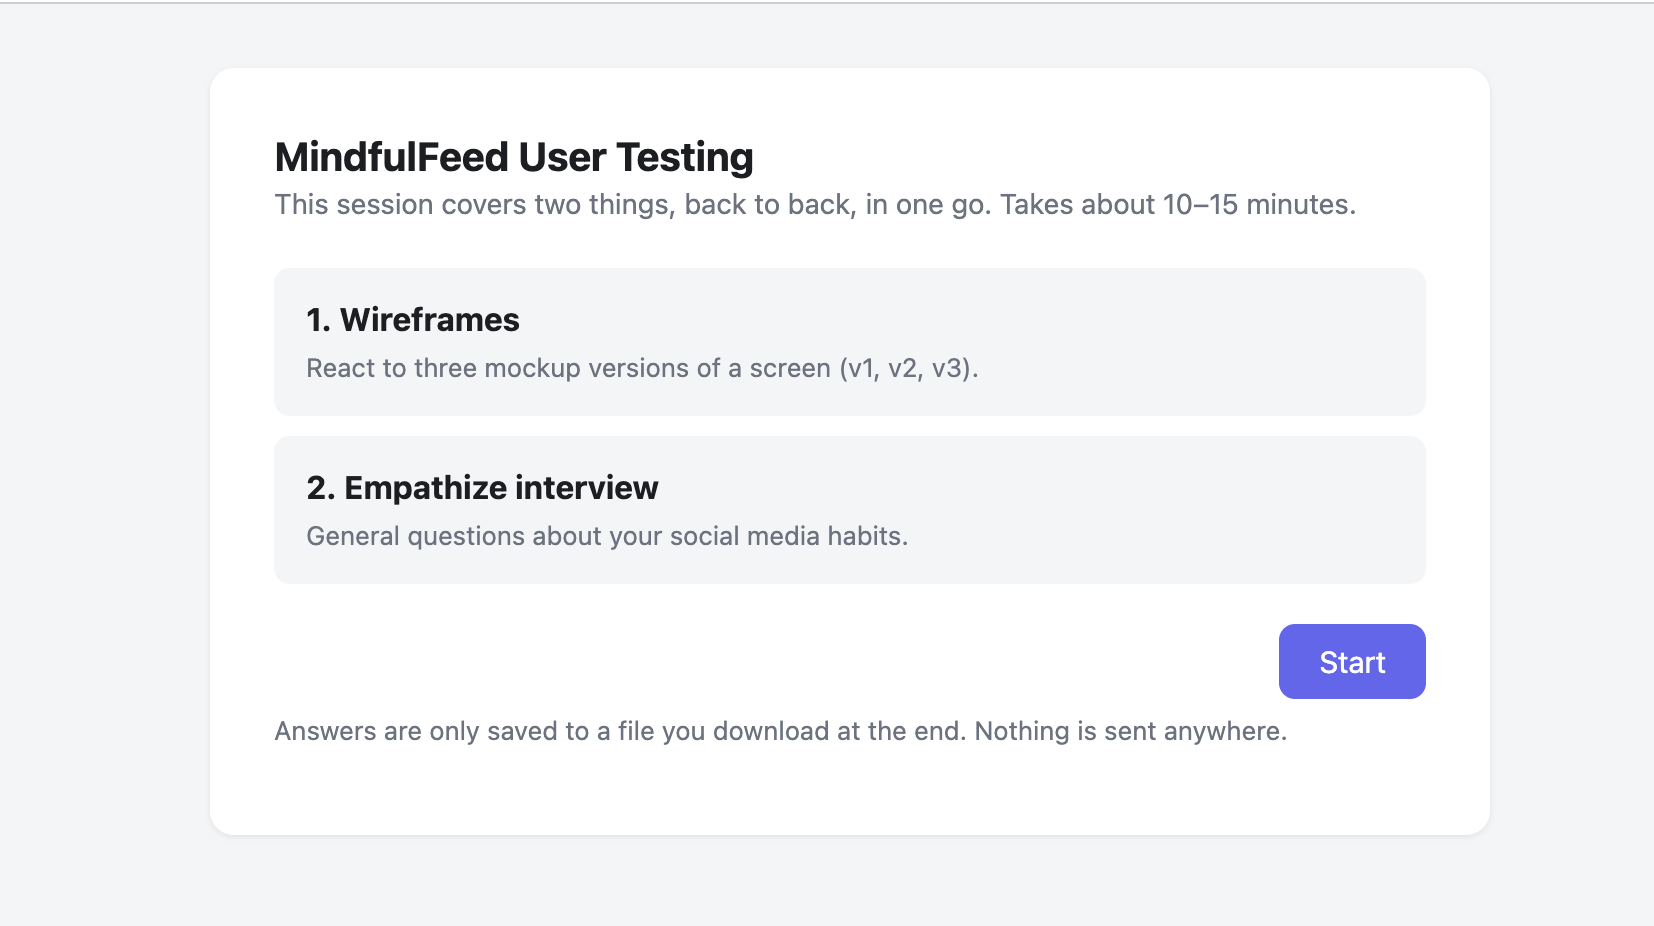
\includegraphics[width=0.8\textwidth,keepaspectratio]{tools/APP IMAGES/Screenshot 2026-09-23 at 22.47.17.png}
\caption{Real-user testing tool: screen 1}
\label{fig:testing_tool_screenshot_1}
\end{figure}

\begin{figure}[H]
\centering
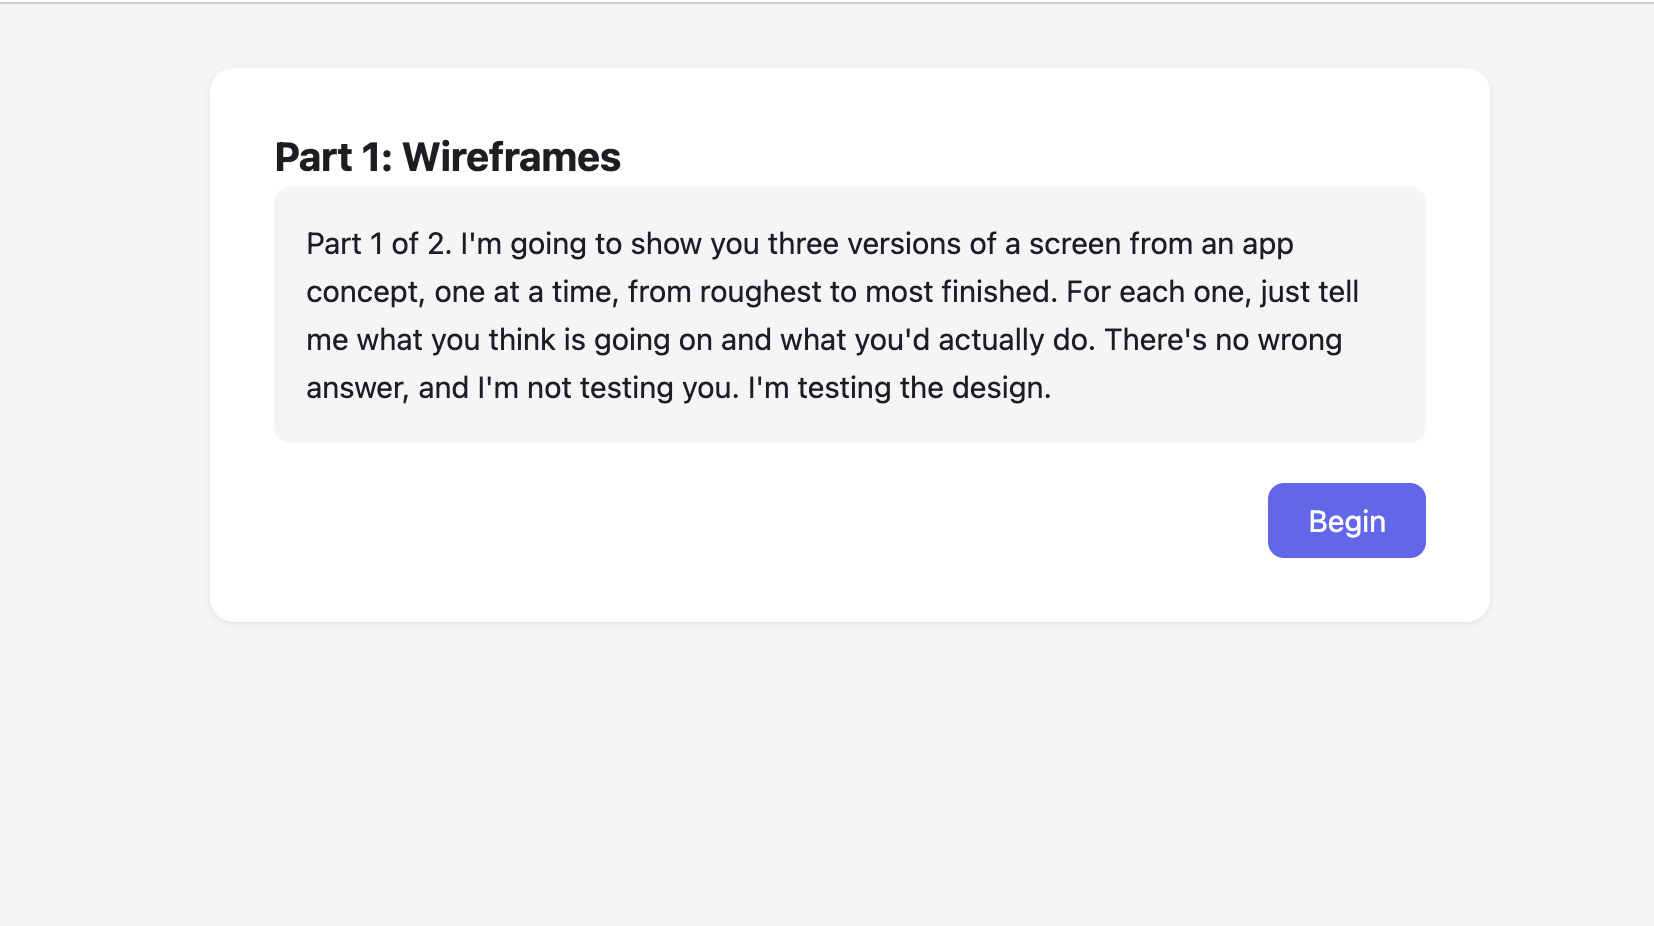
\includegraphics[width=0.8\textwidth,keepaspectratio]{tools/APP IMAGES/Screenshot 2026-09-23 at 22.47.26.png}
\caption{Real-user testing tool: screen 2}
\label{fig:testing_tool_screenshot_2}
\end{figure}

\begin{figure}[H]
\centering
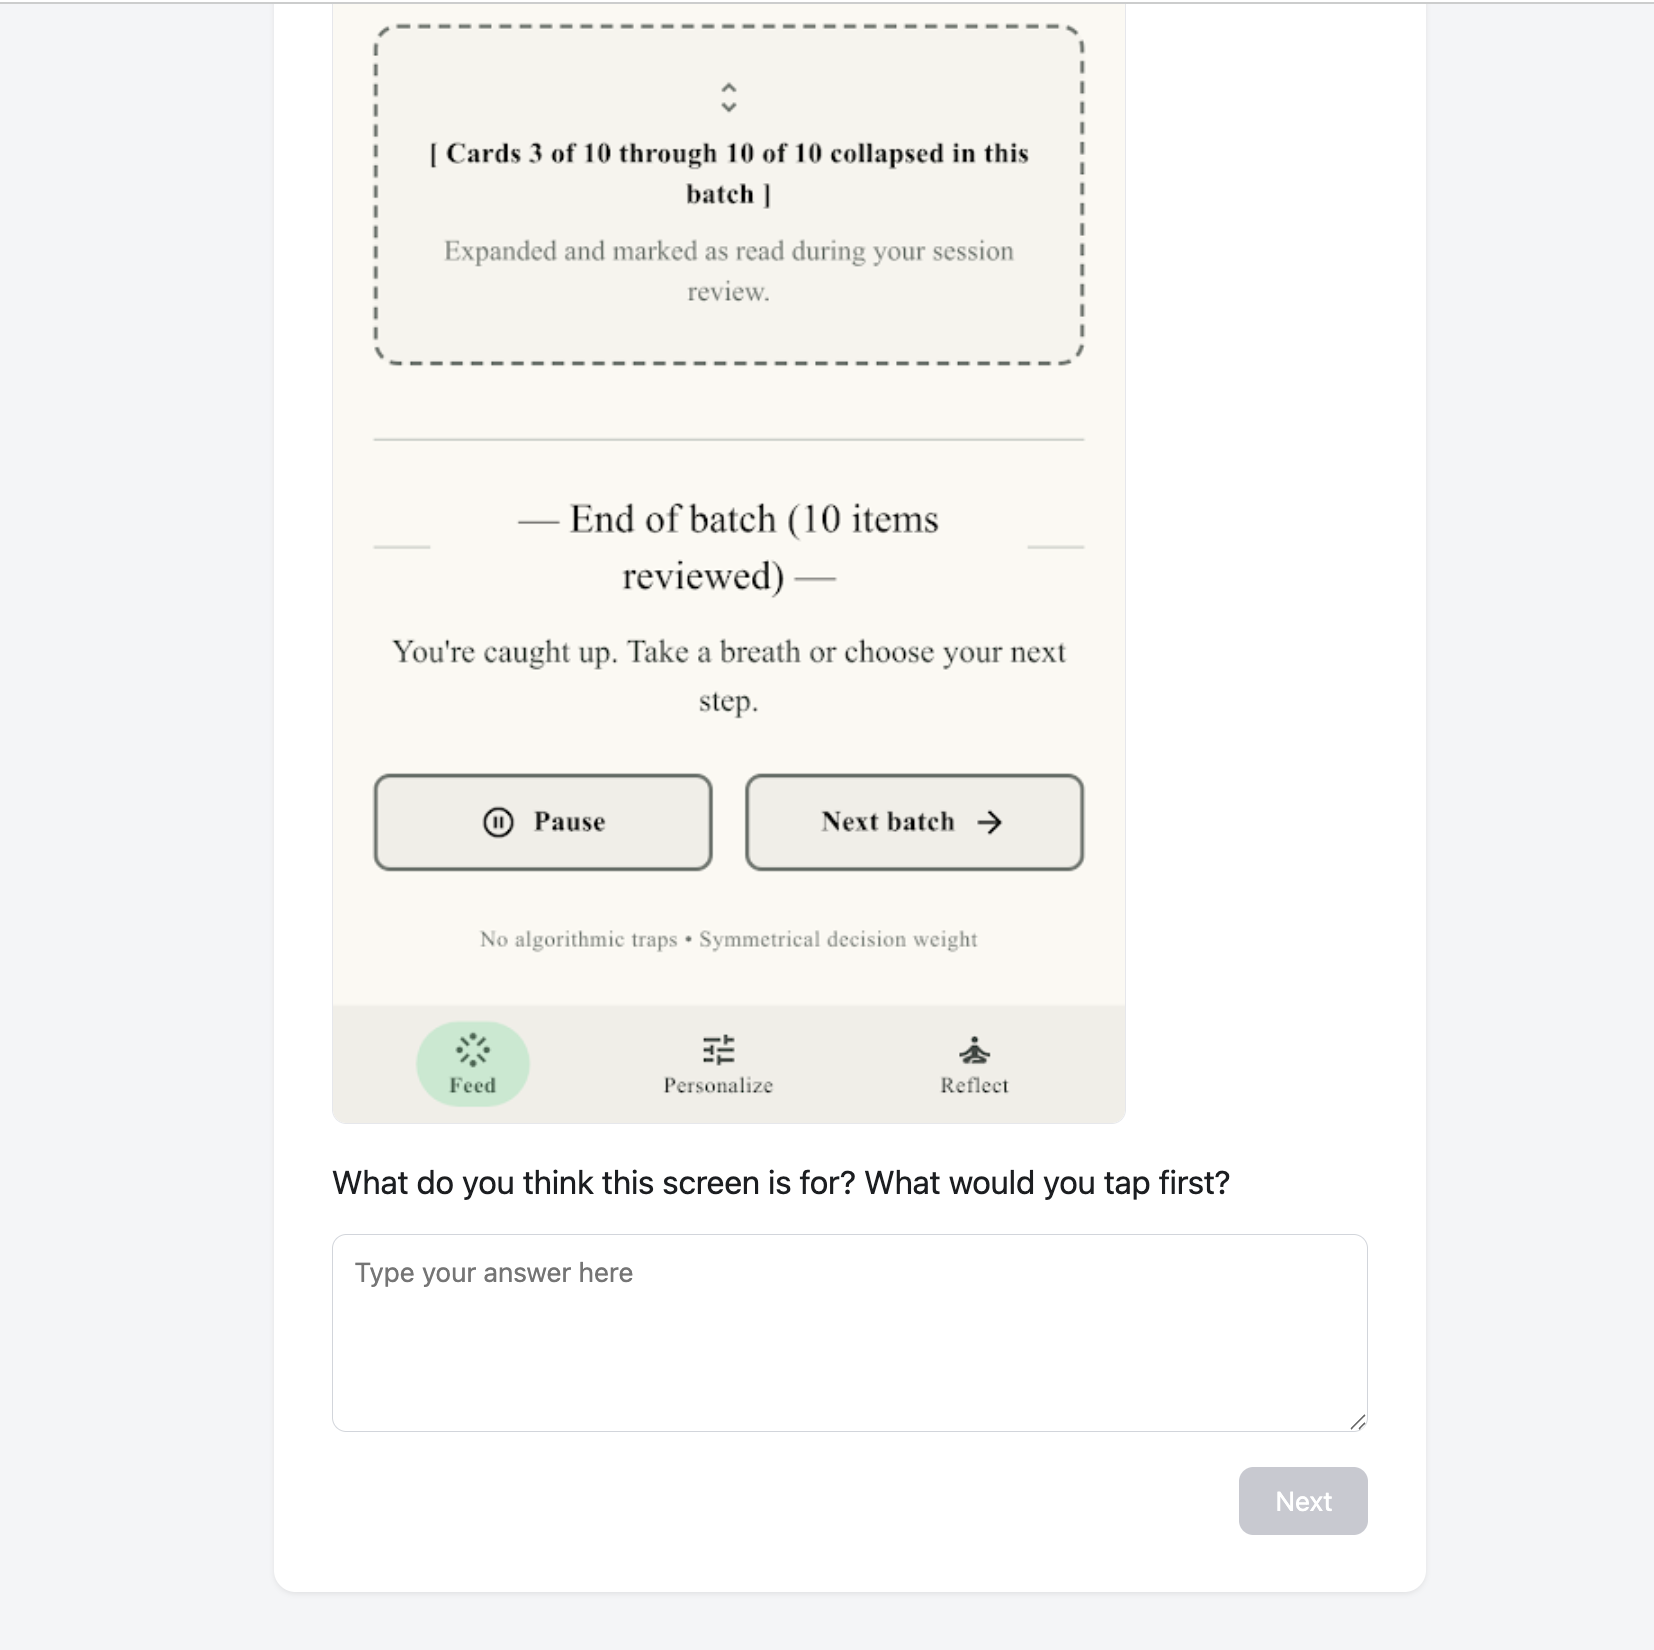
\includegraphics[width=0.8\textwidth,keepaspectratio]{tools/APP IMAGES/Screenshot 2026-09-23 at 22.56.16.png}
\caption{Real-user testing tool: screen 3}
\label{fig:testing_tool_screenshot_3}
\end{figure}

\begin{figure}[H]
\centering
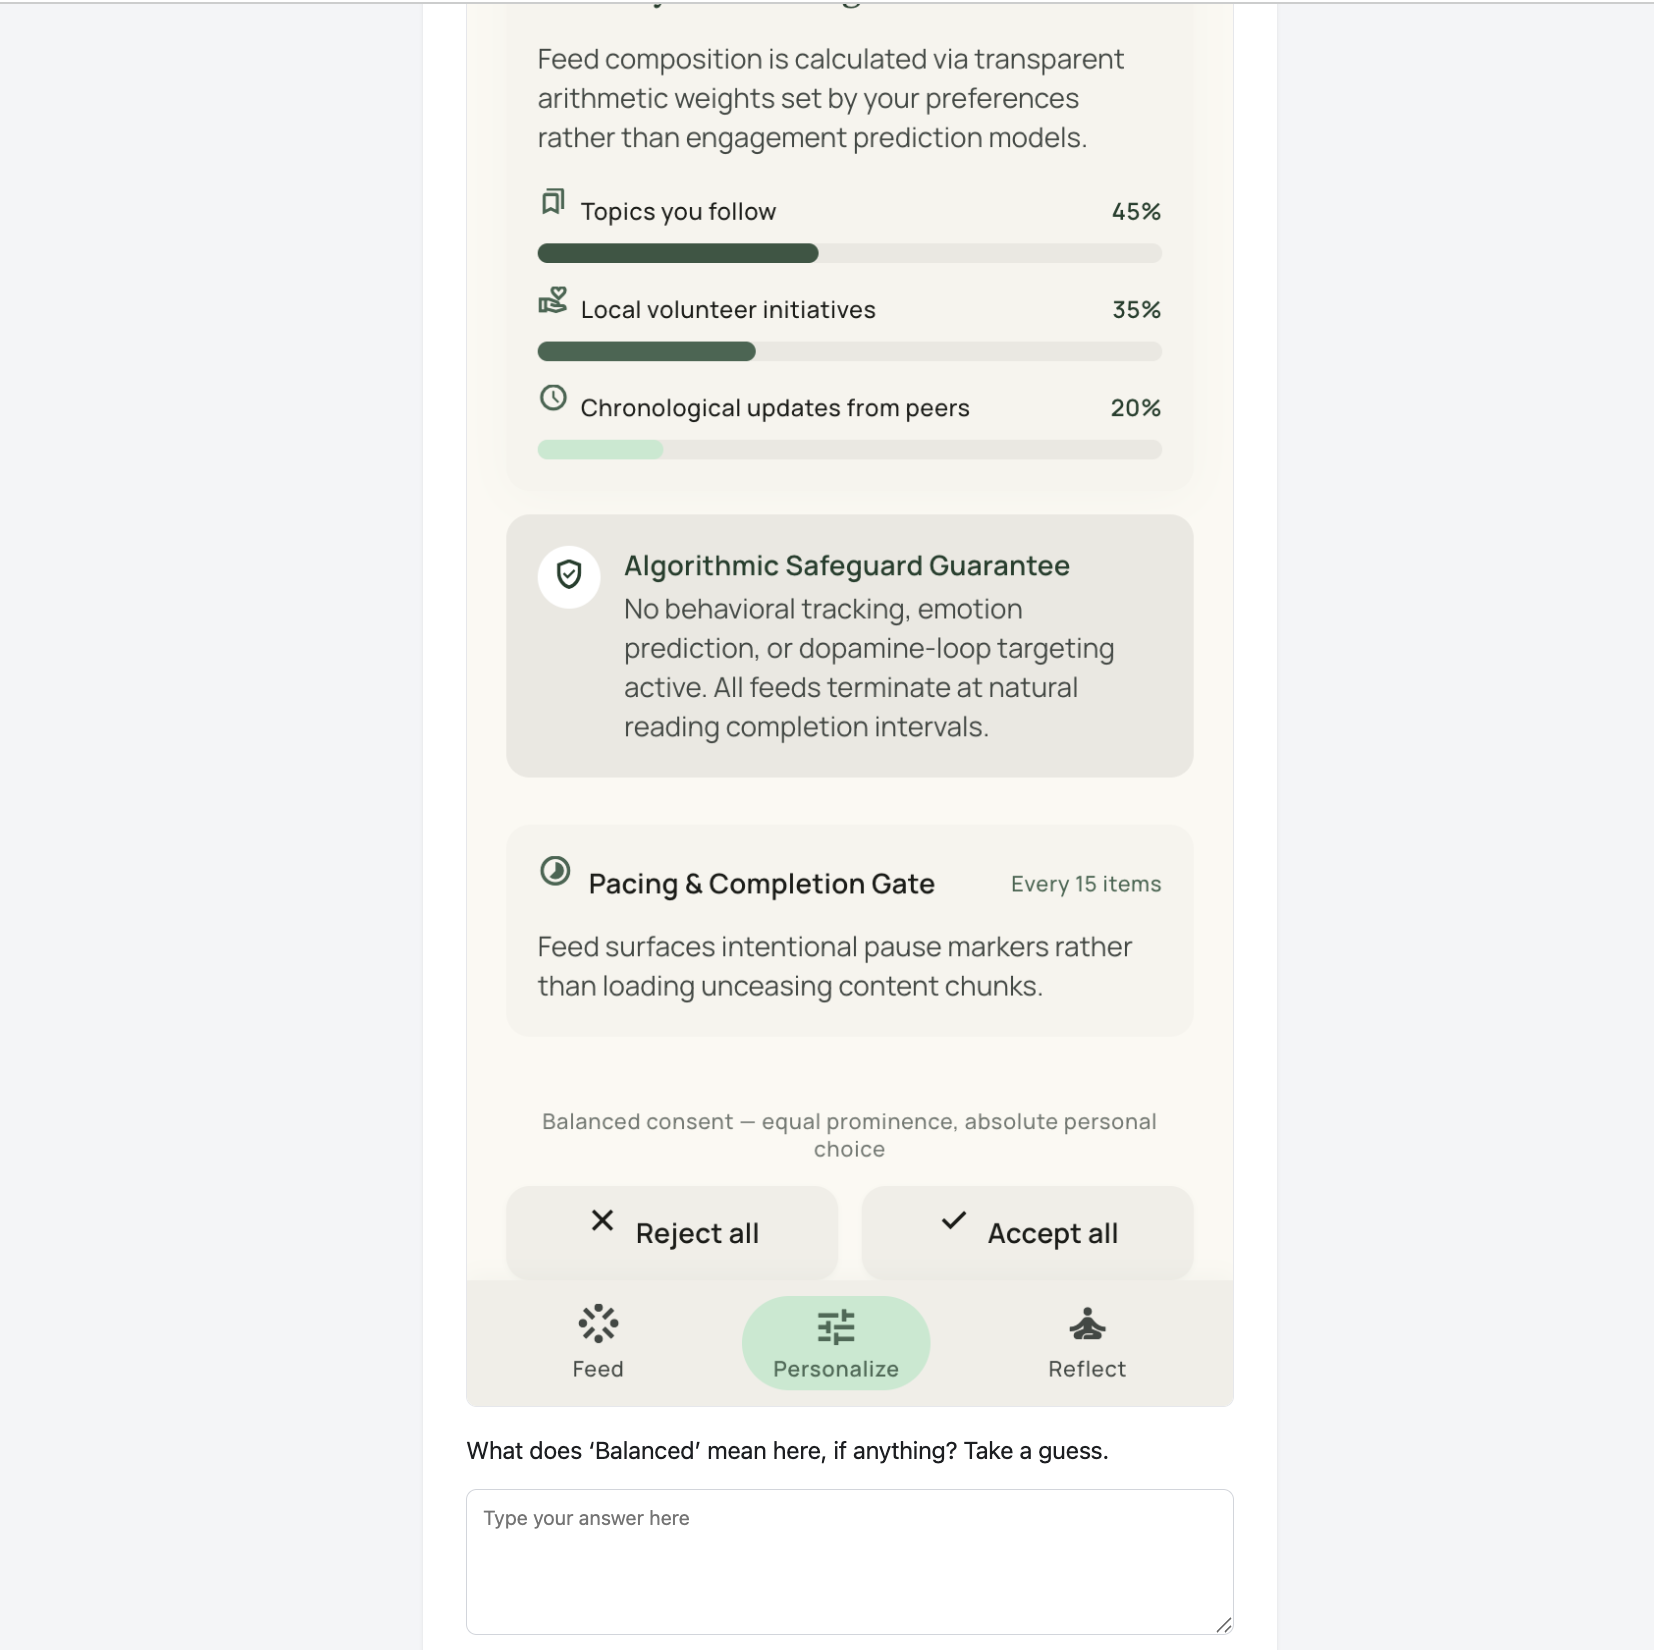
\includegraphics[width=0.8\textwidth,keepaspectratio]{tools/APP IMAGES/Screenshot 2026-09-23 at 22.56.41.png}
\caption{Real-user testing tool: screen 4}
\label{fig:testing_tool_screenshot_4}
\end{figure}

\begin{figure}[H]
\centering
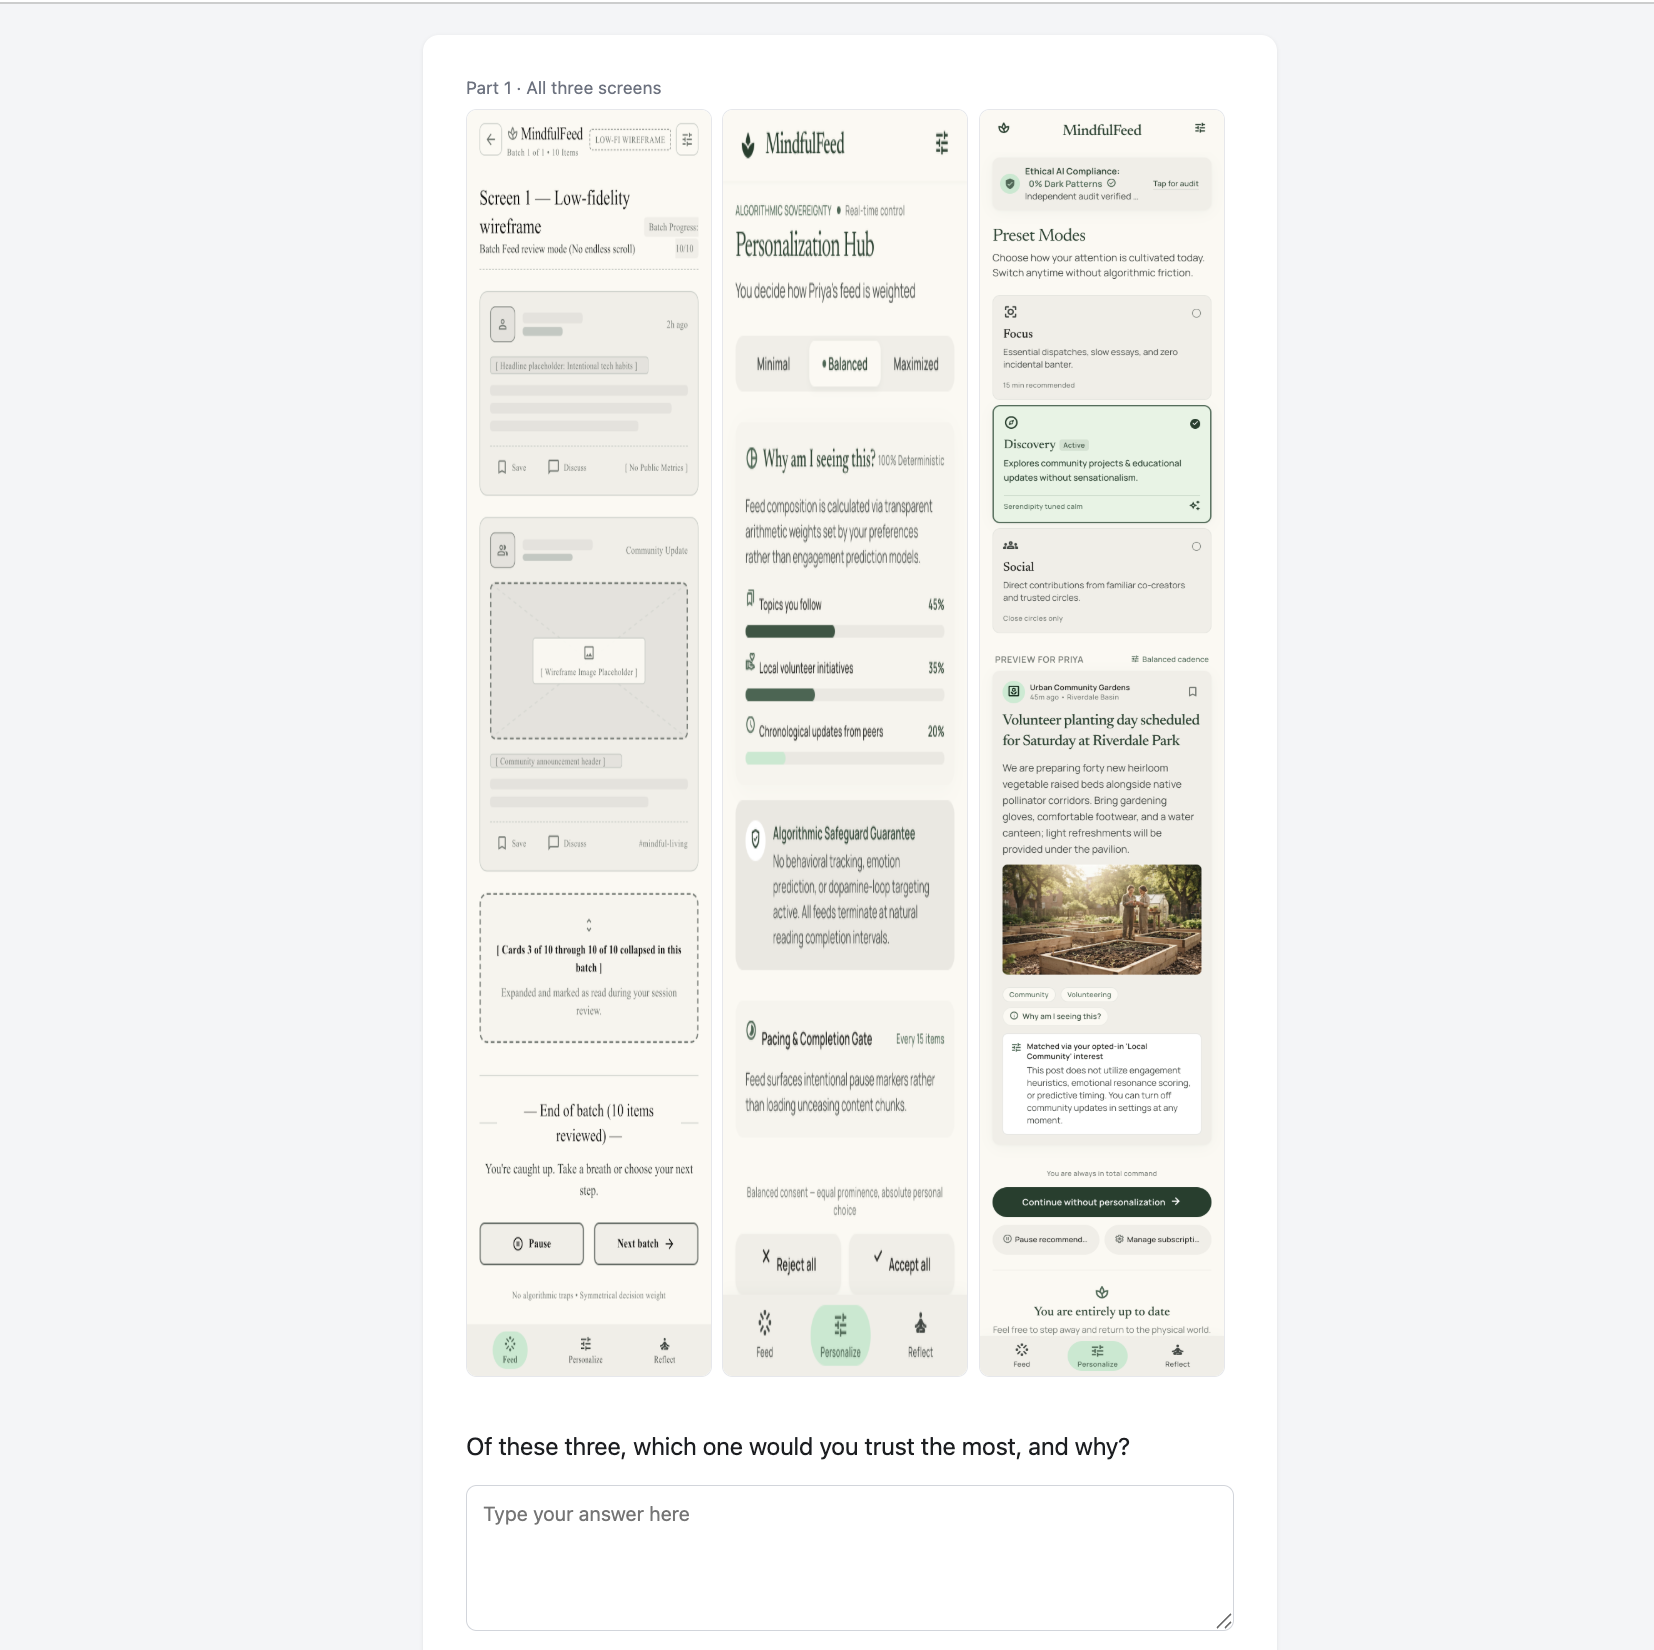
\includegraphics[width=0.8\textwidth,keepaspectratio]{tools/APP IMAGES/Screenshot 2026-09-23 at 22.57.01.png}
\caption{Real-user testing tool: screen 5}
\label{fig:testing_tool_screenshot_5}
\end{figure}

\begin{figure}[H]
\centering

\includegraphics[width=0.8\textwidth,keepaspectratio]{tools/APP IMAGES/Screenshot 2026-09-23 at 22.57.13.png}
\caption{Real-user testing tool: screen 6}
\label{fig:testing_tool_screenshot_6}
\end{figure}

\begin{figure}[H]
\centering
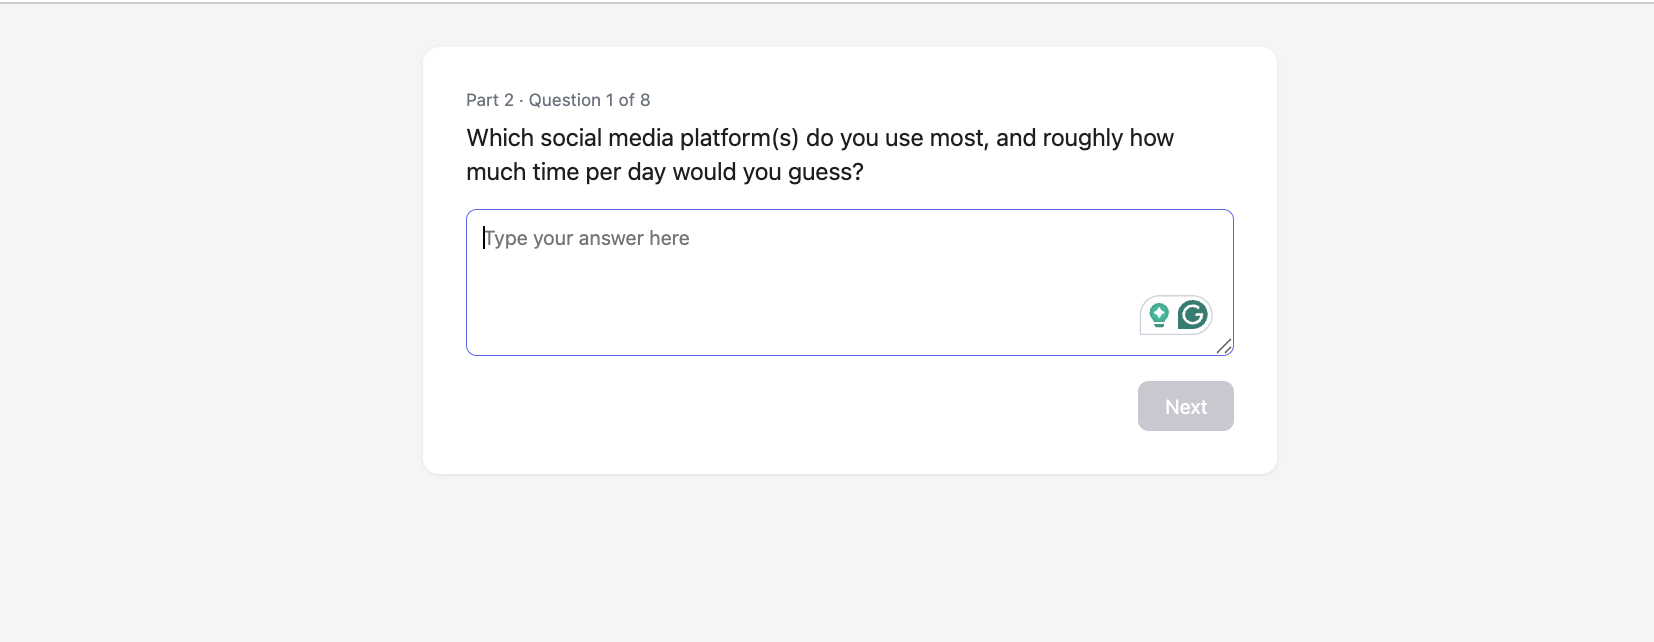
\includegraphics[width=0.8\textwidth,keepaspectratio]{tools/APP IMAGES/Screenshot 2026-09-23 at 22.57.19.png}
\caption{Real-user testing tool: screen 7}
\label{fig:testing_tool_screenshot_7}
\end{figure}

\begin{figure}[H]
\centering
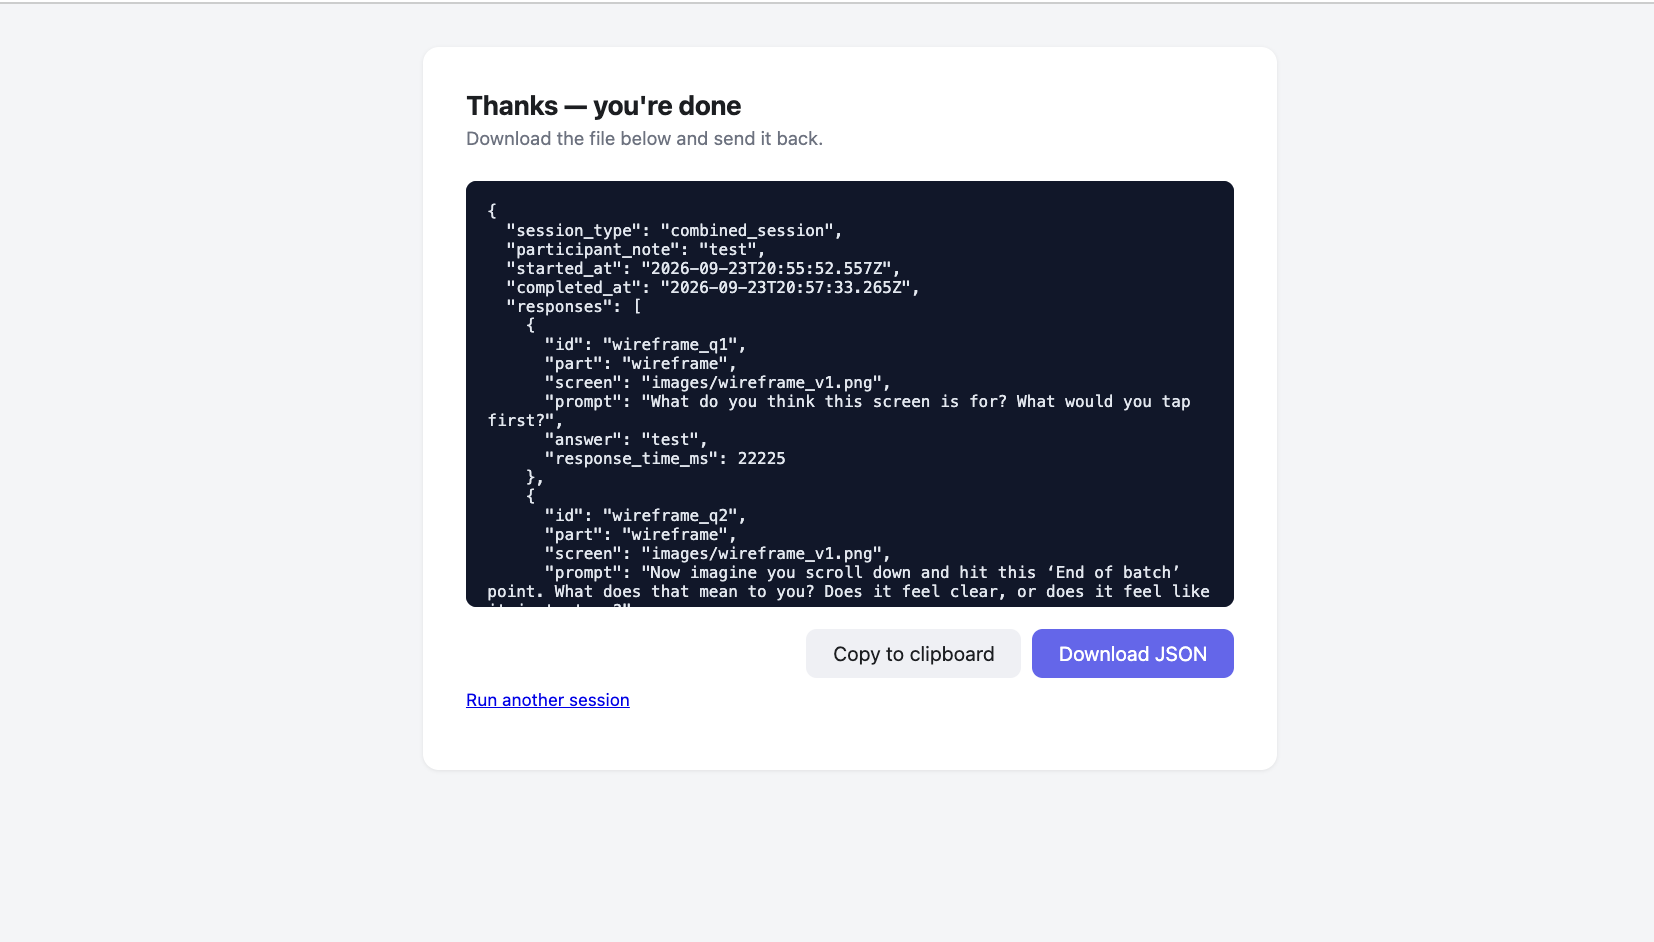
\includegraphics[width=0.8\textwidth,keepaspectratio]{tools/APP IMAGES/Screenshot 2026-09-23 at 22.57.39.png}
\caption{Real-user testing tool: screen 8}
\label{fig:testing_tool_screenshot_8}
\end{figure}

\end{document}
